\documentclass[12pt, a4paper]{report}
\usepackage{a4wide}

\usepackage[english]{babel}
%\usepackage[backend=bibtex]{biblatex}
%\addbibresource{bibliography.bib}

% Setează spațiere inter-linie la 1.5
\usepackage{setspace}
%\onehalfspacing

% Modificarea geometriei paginii
\usepackage{geometry}
% Include funcțiile de grafică
\usepackage{graphicx}
% Încarcă imaginile din directorul `images`
\graphicspath{{./images/}}
% Listări de cod
\usepackage{listings}

% Linkuri interactive în PDF
\usepackage[
    colorlinks,
    linkcolor={black},
    menucolor={black},
    citecolor={black},
    urlcolor={blue}
]{hyperref}


% Suport pentru rezumat în două limbi
% Bazat pe https://tex.stackexchange.com/a/70818
\newenvironment{abstractpage}
  {\cleardoublepage\vspace*{\fill}\thispagestyle{empty}}
  {\vfill\cleardoublepage}
\renewenvironment{abstract}[1]
  {\bigskip
  \begin{center}\bfseries\abstractname\end{center}}
  {\par\bigskip}


% Suport pentru anexe
\usepackage{appendix}

% Stiluri diferite de headere și footere
\usepackage{fancyhdr}

\fancypagestyle{front}{
  \fancyhf{}
  \renewcommand{\headrulewidth}{0pt}
  \cfoot{}
}
\fancypagestyle{main}{
  \fancyhf{}
  \renewcommand\headrulewidth{0pt}
  \fancyhead[C]{}
  \fancyfoot[C]{\thepage}
}

% for code snipets
\usepackage{minted}

% for multiple columns
\usepackage{multicol}
\usepackage{subfigure}
\usepackage{rotating}
\usepackage{subfloat}

\def\code#1{\texttt{#1}}

\title{Design and Implementation of an automated form generation and parsing tool}
\author{Theodor Pierre Moroianu}

% Generează variabilele cu @
\makeatletter

\begin{document}

% Front matter
\cleardoublepage
\pagestyle{front}
\let\ps@plain\ps@front

% Pagina de titlu
\begin{titlepage}

  % Redu marginile
  \newgeometry{left=2cm,right=2cm,bottom=1cm}
  
  \begin{figure}[!htb]
      \centering
      \begin{minipage}{0.2\textwidth}
          
\includegraphics[width=\linewidth]{logo-ub.png}
      \end{minipage}
      \begin{minipage}{0.5\textwidth}
          \large
          \vspace{0.2cm}
          \begin{center}
              \textbf{UNIVERSITATEA DIN BUCUREȘTI}
          \end{center}
          \vspace{0.3cm}
          \begin{center}
              \textbf{
                  FACULTATEA DE \\
                  MATEMATICĂ ȘI INFORMATICĂ
              }
          \end{center}
      \end{minipage}
      \begin{minipage}{0.2\textwidth}
          
\includegraphics[width=\linewidth]{logo-fmi.png}
      \end{minipage}
  \end{figure}
  
  \begin{center}
  \textbf{SPECIALIZAREA INFORMATICĂ}
  \end{center}
  
  \vspace{1cm}
  
  \begin{center}
  \Large \textbf{Lucrare de licență}
  \end{center}
  
  \begin{center}
  \huge \textbf{\MakeUppercase{\@title}}
  \end{center}
  
  \vspace{3cm}
  
  \begin{center}
  \large \textbf{Absolvent \\ \@author}
  \end{center}
  
  \vspace{0.25cm}
  
  \begin{center}
  \large \textbf{Coordonator \c{S}tiințific \\ Alin \c{S}tef\u{a}nescu}
  \end{center}
  
  \vspace{2cm}
  
  \begin{center}
  \Large \textbf{București, Iunie 2022}
  \end{center}
\end{titlepage}

\restoregeometry
\restoregeometry
\newgeometry{
    margin=2.5cm
}

\addtocounter{page}{1}

% Rezumatul
\begin{abstractpage}

  \begin{abstract}{}
  Am g\u{a}ndit \c{s}i implementat serverul unei aplica\c{t}ii de creare, gestionare \c{s}i parsare automat\u{a} a formularelor. Produsul complet este API-ul utilizat de o aplica\c{t}ie web modern\u{a} (web 2.0), care ofera urmatoarele functionalita\c{t}i: autentificarea utilizatorilor folosind \textit{OAuth2}, generarea formularelor \c{s}i descarcarea acestora \^{i}n format PDF, completarea formularelor online, extragerea automat\c{a} a raspunsurilor din pozele unui formular imprimat, c\^{a}t \c{s}i control deplin (citire / creare / modificare / \c{s}tergere) asupra formularelor \c{s}i a r\u{a}spunsurilor.
  
  \^{I}mpreun\u{a} cu aplica\c{t}ia client (implementat\u{a} in cadrul altui proiect), produsul nostru constituie o alternativ\u a a serviciilor precum \textit{Google Forms} sau \textit{Microsoft Forms}. Aplica\c tia este disponibil\u a pe internet la adresa \textit{https://smartforms.ml}, dar poate fi \c si g\u azduit\u a local -- codul este open-source \c si distribuit sub o licen\c t\u a \textit{MIT} permisiv\u a. Prin capacitatea acesteia de-a citi \c si parsa formulare imprimate \c si completate de m\^ an\u a, aplica\c tia este ideal\u a pentru profesori, secretariate sau oricine av\u and de digitalizat cantita\c ti mari de date. 
  
  \end{abstract}
  
  \begin{abstract}{}
  I designed and implemented the backend of an app focused on the creation and management of forms and surveys. The final product is the API server used by a \textit{Web 2.0} application, offering the following functionality: user authentication (using \textit{OAuth 2}),creation of forms and the ability to download them as PDF documents, filling forms online, extracting answers from pictures or scans of filled forms, and CRUD control over forms and answers.
  
  Together with the client app (which was implemented within another project), our software is an alternative to online websites such as \textit{Google Forms} or \textit{Microsoft Forms}. The application is accessible online at \textit{https://smartforms.ml}, but can be also ran locally -- the code is open-source and distributed under a permissive \textit{MIT} licence. Thanks to its ability to digitize printed forms, our software is especially useful to to teachers, receptions or anywhere massive amounts of digitisation are required.
  \end{abstract}
  
\end{abstractpage}

\tableofcontents

% Main matter
\cleardoublepage
\pagestyle{main}
\let\ps@plain\ps@main


% explic pe scurt ce face aplicatia.
% explic din perspectiva userului, fara
% sa dau detalii despre tech side
\chapter{Introduction}

\section{Functionality}

Our project, called \textit{SmartForms} is centered around creating and digitization of forms, for minimizing human intervention. By using the software we created, users can, between others:
\begin{itemize}
    \item Create simple forms, in a PDF format, prompting readers to fill in multiple choice questions or manually writing answers.
    \item Upload scans of filled forms, which are then automatically parsed and added to the list of answers.
    \item Share the link to an online form, similar to modern survey websites.
    \item Fully control (View / Edit / Delete) forms and answers.
\end{itemize}

\section{Use Case and Target Audience}

The main use case of this software is situations where massive amounts of physical data need to be digitized to be further processed, or, due to legal or connectivity issues, alternatives like \textit{Google Forms} or \textit{Microsoft Forms} are not an option.

Due to the its high flexibility, our software aims to solve the given scenarios:

\subsection*{Scenario 1: Written Exams}

A teacher wants to organize an exam for a large number of students.\\
The exam is comprised of questions which are either multiple choice, either with a restrained set of possible answers (e.g. for a geography course, an answer could be "\textit{Paris}", or for a mathematics course a possible answer would be "$3.1415$").

The teacher doesn't want to give his/her students access to the internet, to avoid fraud, so an online form isn't feasible. On the other hand, a written exam means the teacher has to manually go throughout each exam paper.

Our software gives the teacher two options:
\begin{enumerate}
    \item Host the software's server locally, letting students connect to the local network without them accessing the internet, and having them submit their answers via our online form submission service.
    \item Create and print the exam using our form generation tool, and have the students fill their answers on a printed copy of the form. Then upload a scan of their answers and let the software extract them.
\end{enumerate}

\subsection*{Scenario 2: Covid-19 Tracking}

While entering institutions such as hospitals, for legal reasons people are asked to fill a simple form with their name, address and contact information.

In case of emergency, workers have to manually go throughout each form to contact the people concerned.

Using our software, workers can simply upload a scan of the filled forms, and download the entire list of email addresses, making contacting the affected people easier and more reliable.

\subsection*{Scenario 3: Data Protection Legal Issues}

With the recent GDPR regulations, data protection is becoming for many companies one of the top priorities.

In this scenario, our software aims to replace online forms or endless email mailing lists, providing a simple, self-contained and self-hosted solution for companies which do not want to use 3rd party questionnaire solutions.

\section{Scope of the Project}

The software is made in collaboration with another student from my cohort.

The complete software is made out of three main components:
\begin{itemize}
    \item The API server, receiving and answering to requests.
    \item The Client, running on the users' browsers as a modern web application.
    \item The environment, connecting the two services from above and making the app visible online.
\end{itemize}

My project's scope is the API server and the services behind it. It includes:
\begin{itemize}
    \item Implementing the API routes.
    \item Implementing the form generation pipeline.
    \item Setting up the database management system.
    \item Implementing the parsing pipeline, extracting answers from scanned forms.
    \item Implementing the authentication mechanism, to allow for different confidentiality levels.
\end{itemize}

My project does NOT include:
\begin{itemize}
    \item Implement any user-facing elements.
    \item Connecting the two services or exposing the application to the internet.
\end{itemize}


\section{Related Work}


% Explic toate tehnologiile folosite, si
% la ce ne ajuta.
\chapter{Tech Stack}

\section{Programming Language}

The primary programming language used in the backend is \textit{Python 3}.
\textit{Python 3} offers a great flexibility, native support for essential datastructures used in web development such as \textit{JSON} (JavaScript Object Notation) and easy to follow syntax.

The main reason we chose \textit{Python} over more conventional languages for web servers is the abundance of packages available to install via \textit{Pip}, the Python Package Manager.

The main drawback of \textit{Python} is its speed. Being an interpreted language it is slower than traditional languages such as \textit{C/C++} or \textit{Java}.

To illustrate the speed difference, we ran a simple program in both \textit{Python} and \textit{C++}, to see the difference.

The \textit{Python} code is:

\definecolor{bg}{rgb}{0.95,0.95,0.95}
\begin{minted}[bgcolor=bg]{Python}
N = 300000

primes = []

for i in range(2, N):
    is_prime = True
    for d in primes:
        is_prime = is_prime and i % d != 0
    if is_prime:
        primes.append(i)

print(f"There are {len(primes)} prime numbers up to {N}")
\end{minted}

The \textit{C++} code, running the exact same instructions is:
\definecolor{bg}{rgb}{0.95,0.95,0.95}
\begin{minted}[bgcolor=bg]{C++}
#include <bits/stdc++.h>
using namespace std;

int main()
{
    int N = 300'000;
    vector <int> primes;

    for (int i = 2; i < N; i++) {
        bool is_prime = true;
        for (auto d : primes)
            is_prime = is_prime && (i % d);
        if (is_prime)
            primes.push_back(i);
    }

    cout << "There are " << primes.size()
        << " prime numbers up to " << N << '\n';
}
\end{minted}

Running them gives us:
\begin{minted}[bgcolor=bg]{Shell}
teo@fedora ~/P/T/L/tech-stack> time python ciur.py
There are 25997 prime numbers up to 300000
________________________________________________________
Executed in  173.56 secs    fish           external
   usr time  173.12 secs  992.00 micros  173.12 secs
   sys time    0.03 secs    0.00 micros    0.03 secs

teo@fedora ~/P/T/L/tech-stack> g++ -O2 ciur.cpp -o ciur-cpp
teo@fedora ~/P/T/L/tech-stack> time ./ciur-cpp
There are 25997 prime numbers up to 300000
________________________________________________________
Executed in    2.57 secs    fish           external
   usr time    2.56 secs  896.00 micros    2.56 secs
   sys time    0.00 secs    0.00 micros    0.00 secs
\end{minted}

In other words, \textit{Python} runs our (quite naive) prime counting algorithm $60$ times slower than the same \textit{C++} code!

While this might seem problematic, in practical cases the difference is less noticeable, and most of our server's computing time is spent by libraries like \textit{OpenCV} or \textit{Numpy}, which are implemented in \textit{C++}, essentially offering us \textit{C++} speeds in \textit{Python}.

\section{Web Server Framework}

The framework we used for implementing the API server is \textit{FastAPI}. \textit{FastAPI} is a scalable, lightweight and efficient \textit{Python} framwork, whose main advantages are:
\begin{itemize}
    \item Automatic validation, serialization and deserialization of the data sent and received by the API endpoints.
    \item Automatic generation of the \textit{OpenAPI} (Swagger) specifications, which can then be used as a reference point for using the API in the frontend.
    \item Asynchronous programming and multiple threads, making it fit for CPU-intensive tasks.
\end{itemize}

\section{Database Management System}

As our application has to store information such as existing users, created forms or answers to a persistent medium, we integrated a database management system to it.

We decided to use \textit{MongoDB}, a document-oriented \textit{NoSQL} system.

\section{Image Manipulation Framework}

For parsing scanned documents, correctly identifying the location of the answers on them and manipulating the images we use \textit{OpenCV}, one of the best computer vision frameworks available together with \textit{Numpy}, the industry standard to data manipulation in \textit{Python}.

While \textit{OpenCV} and \textit{Numpy} are written in \textit{C++} for performance reasons, \textit{Python} bindings allow us to fully use their extensive set of functionality without leaving \textit{Python} land.

\section{Machine Learning Framework}

The parsing part of \textit{SmartForms} is done with the help of machine learning, achieved using a convolutional neural network.

The neural network is implemented in \textit{Pytorch}, one of the best deep learning libraries.




% dau detalii tehnice, cu o explicatie
% printr-o diagrama cum se misca datele
% in aplicatie
\chapter{Design of the Application}


\section{Application Modules}

To simplify the structure of the project and make the code easier to understand, the server is divided into different modules, each one having a different scope (single-responsibility principle). The modules are:
\begin{itemize}
    \item The database module, handling the connection with the \textit{MongoDB} database.
    \item The OCR module, taking care of the neural network and character prediction.
    \item The PDF processor module, which generates and parses the PDF forms.
    \item The router module, handling the API calls.
    \item The storage module, in which internal types are defined.
    \item The testing module, where unit and integration tests are defined.
\end{itemize}


\begin{figure}[!h]
    \centering
    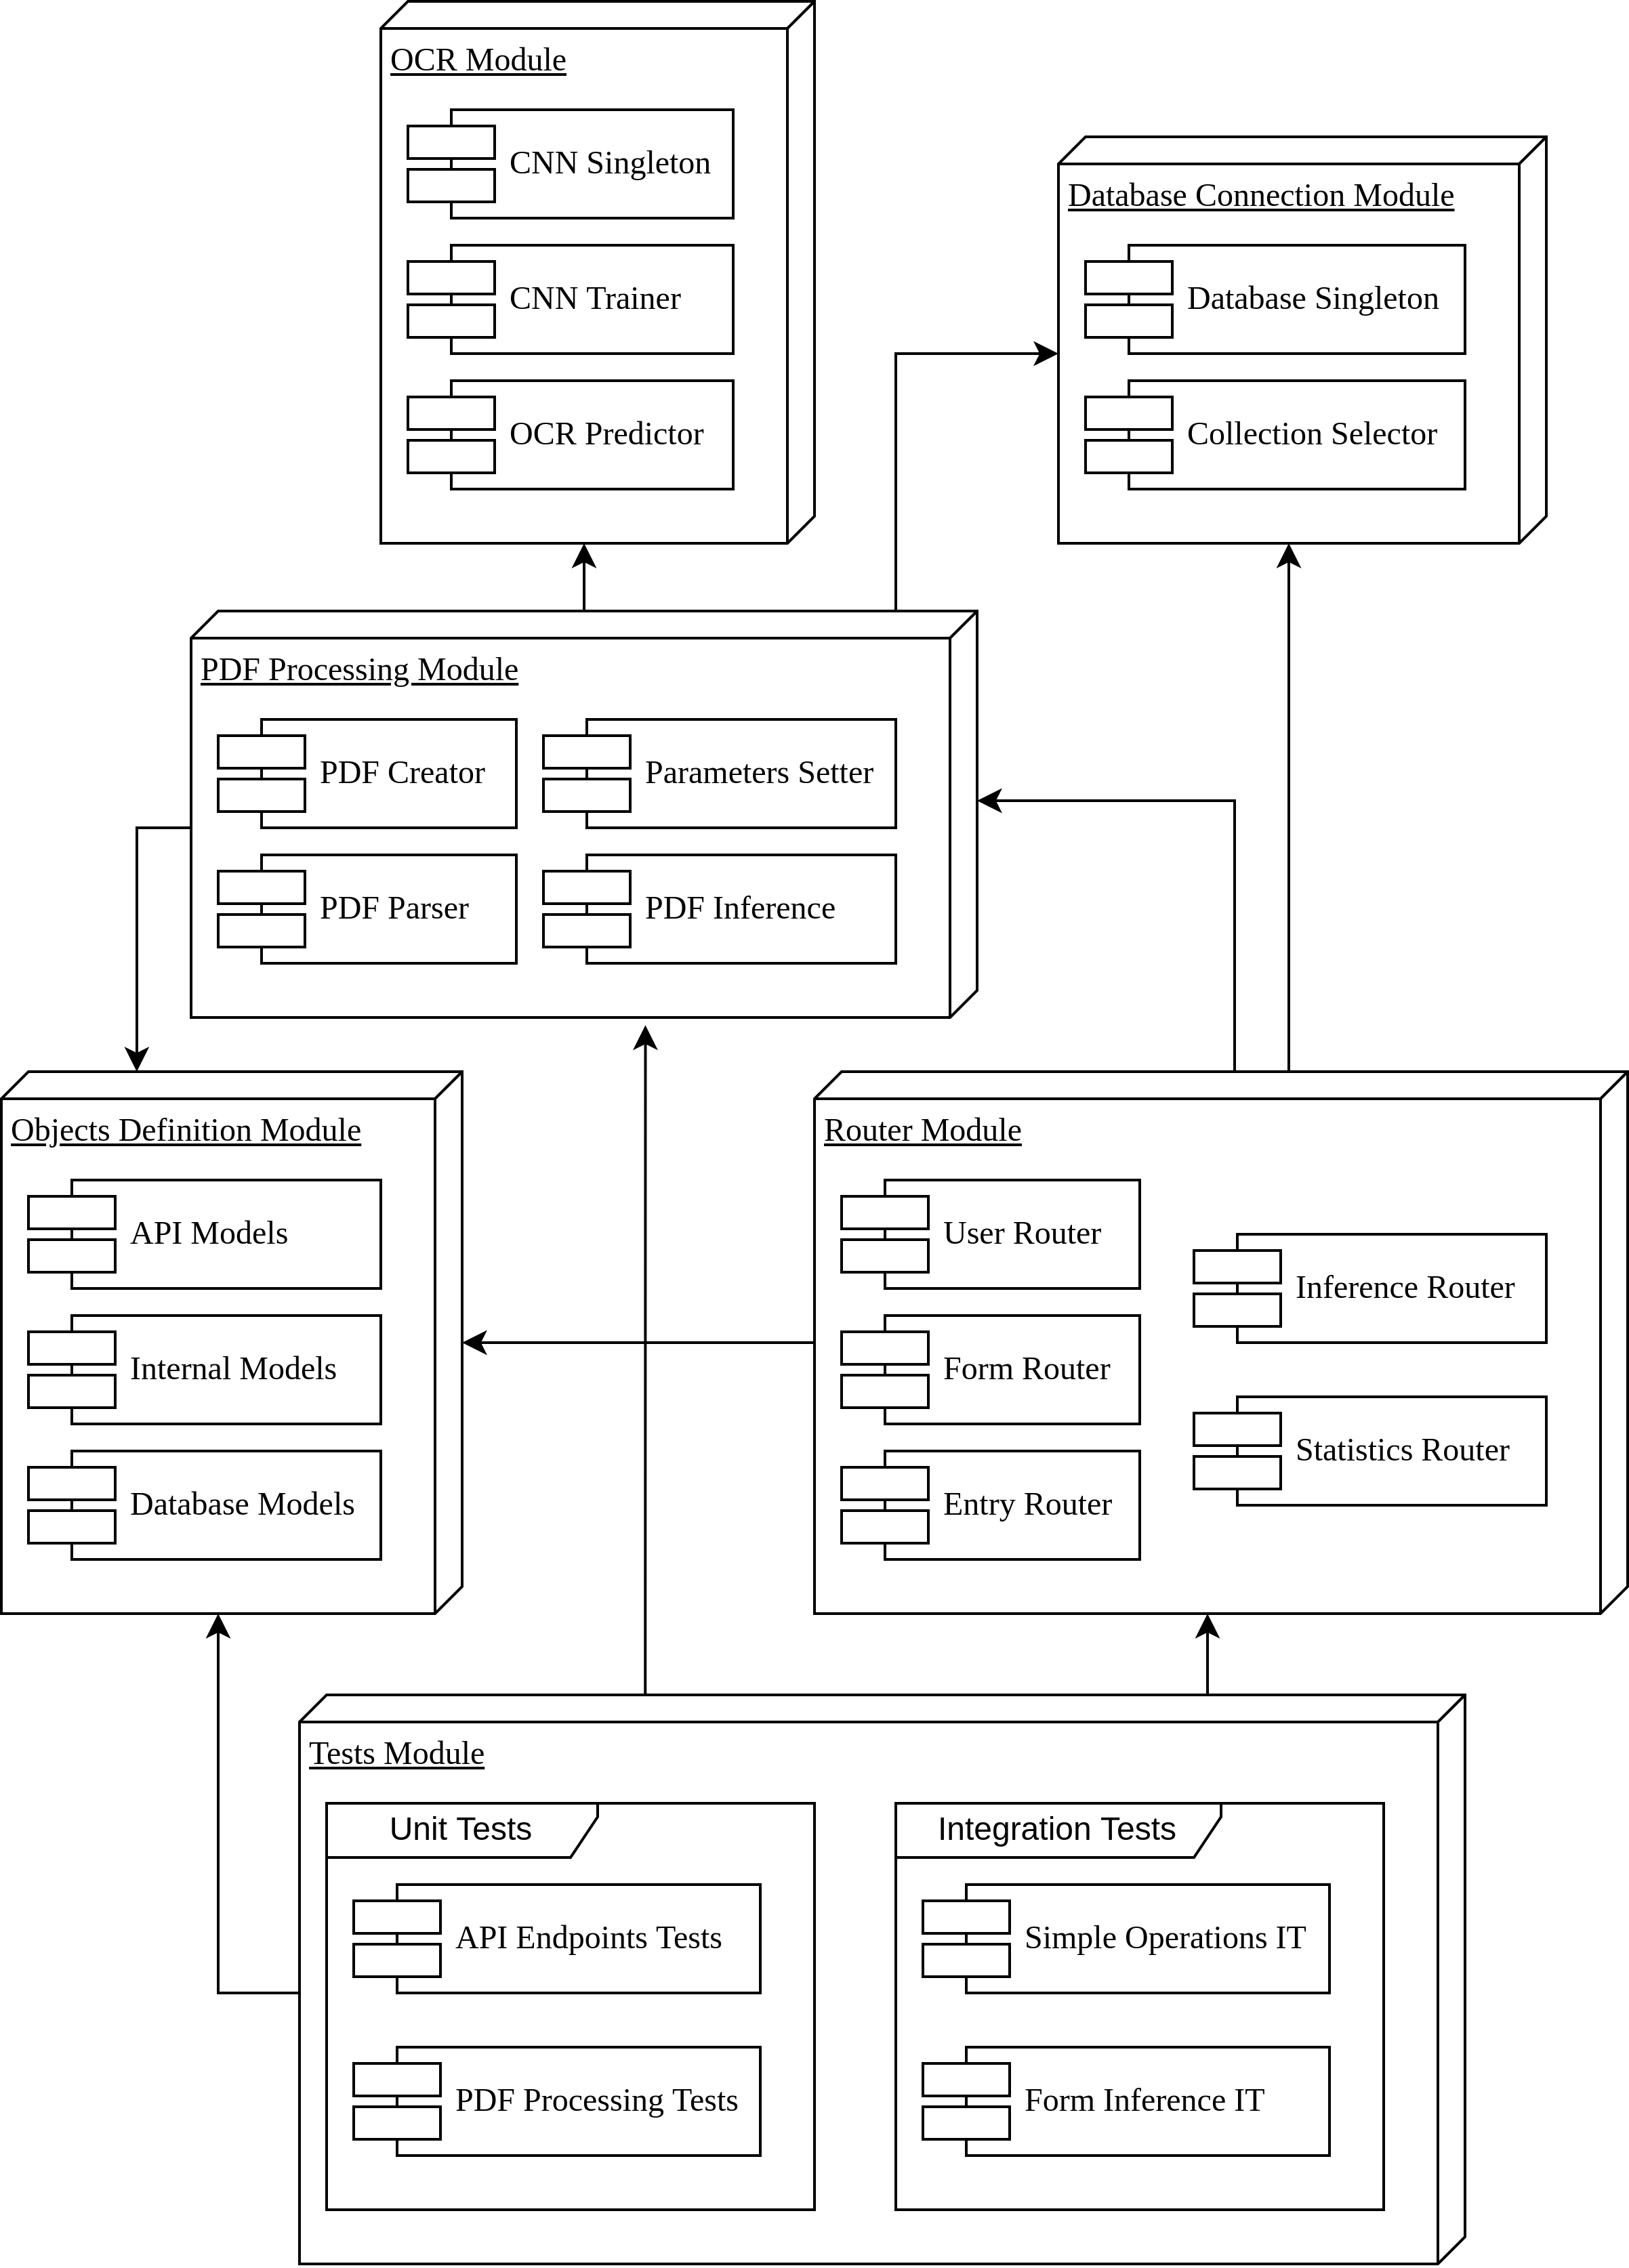
\includegraphics[width=37em]{images/diagrams/ProjectModulesDiagram.png}
    \caption{UML Diagram Of SmartForms's Backend Modules}
    \label{fig:label}
\end{figure}

Each module is designed to act as an independent unit, interacting with the others only with the help of a reduced number of function calls / \textit{Singleton} interfaces.

Modules are written according to the standard \textit{Python} conventions:
\begin{itemize}
    \item The source files for each module is located in a folder with the module's name.
    \item At the root of the folder, a file named \code{\_\_init\_\_.py} is created. This file is then populated with all of the functionalities the module needs to export.
\end{itemize}

A sample \code{\_\_init\_\_.py} file is:

\definecolor{bg}{rgb}{0.95,0.95,0.95}
\begin{minted}[bgcolor=bg]{Python}
# backend/sources/smart_forms_types/__init__.py
"""
Types used for storing / processing documents.
"""

import uuid

def generate_uuid():
    """
    generates an unique ID.
    the probability of collisions between different
    uuids is beyond negligable.
    """
    return str(uuid.uuid1())

from smart_forms_types.pdf_form import *
from smart_forms_types.models import *
from smart_forms_types.user import *
from smart_forms_types.inference_dataset import *
\end{minted}

% explic cum functioneaza aplicatia
\chapter{Detailed Overview of the API}

\section{What is an API, and why do we need one?}

The \textit{API} -- or \textit{Application Programming Interface} is an interface acting like a bridge between applications, essentially allowing for an over-the-network communication between two applications.

The most common form of \textit{API} implementations are made with the help of the \textit{HTTP} protocol, an application-layer protocol on top of \textit{TCP}. For showcasing the utility of using an \textit{API}, we can make a simple request to get the current time:

\definecolor{bg}{rgb}{0.95,0.95,0.95}
\begin{minted}[bgcolor=bg]{Shell}
teom@lapttop ~> curl "http://worldtimeapi.org/api/timezone/Europe/Bucharest"\
                 | python -m json.tool
  % Total    % Received % Xferd  Average Speed   Time    Time     Time  Current
                                 Dload  Upload   Total   Spent    Left  Speed
100   395  100   395    0     0   1220      0 --:--:-- --:--:-- --:--:--  1222
{
    "abbreviation": "EEST",
    "client_ip": "5.12.1.116",
    "datetime": "2022-05-20T12:17:44.160367+03:00",
    "day_of_week": 5,
    "day_of_year": 140,
    "dst": true,
    "dst_from": "2022-03-27T01:00:00+00:00",
    "dst_offset": 3600,
    "dst_until": "2022-10-30T01:00:00+00:00",
    "raw_offset": 7200,
    "timezone": "Europe/Bucharest",
    "unixtime": 1653038264,
    "utc_datetime": "2022-05-20T09:17:44.160367+00:00",
    "utc_offset": "+03:00",
    "week_number": 20
}
\end{minted}

This shell script uses the \textit{curl} program, used for querying content over the network, which:
\begin{enumerate}
    \item Breaks down the \textit{URL} we requested (\code{http://worldtimeapi.org/api/timezone/Europe/Bucharest}) into two components:
    \begin{itemize}
        \item The domain -- \code{http://worldtimeapi.org}, which in turn is changed into an \textit{IP} address with the help of a \textit{DNS} server.
        \item The resource path (or route) -- \code{/api/timezone/Europe/Bucharest}, used by the API server to determine what information we want to receive.
    \end{itemize}
    \item Sends the request to the API server.
    \item Receives back the payload sent by the API server, which is piped into the \textit{Python} \textit{JSON} displaying tool to be easy to read.
\end{enumerate}

In the example above, the \textit{API} function we called doesn't have any side-effects -- it doesn't change the internal state of the server. However, in most practical cases we need to be able to alter the stored information.

\section{SmartForms \textit{API}}

The entire \textit{SmartForms} backend software is aimed at being able to respond to API calls.\\
In this section we will go over all of the available endpoints of the \textit{API}, exposing all of the user-facing functionalities of the application. They are divided into categories, each one determined by its path and served by a different router.

Note that we will only give a short description of the available endpoints (the \textit{HTTP Verb} and the path used). To see additional details such as parameters or security restrictions, please check the resources mentioned in the appendix.

\subsection{User Router}

This router exposes functionalities relating to the authentication, registration and deletion of accounts from the platform.

Its endpoints are:
\begin{itemize}
    \item \code{GET /api/user} -- shows a simple message telling the user if he/she is logged in, and promps it to sign in or sign out.
    \item \code{GET /api/user/login} and code{GET /api/user/auth} -- both endpoints help the user to sign-in / sign-up.
    \item \code{GET /api/logout} -- signs out the user.
    \item \code{DELETE /api/delete-account} -- deletes the user's account, his/her forms and his/her entries.
\end{itemize}

\subsection{Form Router}

The \textit{Form Router} handles the PDF form creation / modification / deletion and retrieval.

Its endpoints are:
\begin{itemize}
    \item \code{POST /api/form/preview} -- receives a description of a form (questions, title, author etc) and returns a preview of the final PDF form. This is especially useful as users tend to try out multiple formats before settling for a form.
    \item \code{POST /api/form/create} -- similar to the \textit{preview} endpoint, but commits the created form to the database.
    \item \code{POST /api/form/list} -- returns a list of available forms, depending on filtering criteria.
    \item \code{GET /api/description/\{formId\}} -- returns the description of a given form.
    \item \code{GET /api/form/pdf/\{formId\}} -- returns the \textit{Base64} encoding of a given PDF form.
    \item \code{DELETE /api/form/delete/\{formId\}} -- deletes the form and all of its associated answers.
    \item \code{PUT /api/form/online-access/\{formId\}} -- updates the visibility of the form (for instance if anyone can submit an answer to it online).
\end{itemize}

Note that it is \textbf{not} possible to change the actual content of a form. This is by design, as having multiple versions of the same form would be a hassle. The \textit{update} of a form is done on the client-side, by simply cloning the description of the initial form and creating a new one.

\subsection{Entry Router}

Similarly to the \textit{Form Router}, the \textit{Entry Router} contains API endpoints manipulating entries (or answers).

Its endpoints are:
\begin{itemize}
    \item \code{POST /api/entry/create} -- adds a new answer to a given form.
    \item \code{DELETE /api/entry/delete/\{entryId\}} -- deletes the entry with the given Id.
    \item \code{PUT /api/entry/edit} -- deletes the entry with the given Id.
    \item \code{GET /api/entry/view-entry/\{entryId\}} -- returns the information provided in the given answer.
    \item \code{POST /api/entry/view-form-entries} -- returns a list of forms respecting a set of given criteria.
\end{itemize}

\subsection{Inference Router}

The single scope of the \textit{Inference Router} is to receive scanned PDF documents, \textit{zip} compressed files, images etc. which are then parsed.

When the software is able to detect a form, it parses it and extracts the answer, which is then added to the database. The endpoint is \code{POST /api/inference/infer}.
\\ \\
Another functionality of the \textit{Inference Router} is to extract character data:
\begin{enumerate}
    \item When an answer is uploaded, the \code{infer} endpoint saves for each character the corresponding sub-image of the answer.
    \item If the answer is later modified by a \code{/api/entry/edit} call, then an annotated character datapoint is generated.
    \item The OCR neural network is trained on the generated dataset.
\end{enumerate}

In other words, if the inference failed, a character is wrongly identified. If someone updates the answer with the correct one, then the software finds the difference and generates a new labeled image it can then use to fine-tune the OCR neural network.

\subsection{Statistics Router}

The \textit{Statistics Router} is aimed at providing additional information about \textit{SmartForms}.

Currently, the only available endpoint is \code{GET /api/statistics/global}, which returns information about the total number of forms and entries, but the router is implemented to simplify adding more advanced statistics in the future.

\section{Usage Scenario}

We will now present a simple usage scenario. We will communicate with the API using the \code{curl} command to better illustrate its functionality, but please note that in normal circumstances users only interact with the client, which performs the API calls in their behalf using the \code{fetch API}.

Let's create a new form, with the title "\textit{Sample Form}", and two questions, one asking for the user's gender and the other for his/her name:

\definecolor{bg}{rgb}{0.95,0.95,0.95}
\begin{minted}[bgcolor=bg]{Shell}
teo@fedora ~> curl -X 'POST' \
                    'http://smartforms.ml:5000/api/form/create' \
                    -H 'accept: application/json' \
                    -H 'Content-Type: application/json' \
                    -d '{
                "title": "Sample Form",
                "description": "Sample form to showcase the API.",
                "questions": [
                  {
                    "title": "Gender",
                    "description": "Boy or Girl",
                    "choices": [
                      "Boy",
                      "Girl"
                    ]
                  },
                  {
                    "title": "Name",
                    "description": "Enter your name, in uppercase.",
                    "maxAnswerLength": 36,
                    "allowedCharacters": "ABCDEFGHIJKLMNOPQRSTUVWXYZ "
                  }
                ],
                "canBeFilledOnline": true,
                "needsToBeSignedInToSubmit": true,
                "creationDate": "2022-05-24T07:29:36.216Z"
              }'
\end{minted}

We get back from the API the following \textit{JSON} object:
\definecolor{bg}{rgb}{0.95,0.95,0.95}
\begin{minted}[bgcolor=bg]{Shell}
{
    "formId": "af61ce94-db35-11ec-a6ed-dca6325bcf52",
    "formPdfBase64": "JVBERi0xLjMKMyAwIG9iago8PC9UeXBl...."
}
\end{minted}

We have now added the form to the database, and received back its Id and a \textit{Base64} encoding of the Pdf document. Let's decode it.

We first have to manually copy the content of the \code{formPdfBase64} field, and we can then run:

\definecolor{bg}{rgb}{0.95,0.95,0.95}
\begin{minted}[bgcolor=bg]{Shell}
    teo@fedora ~> pbpaste | base64 -d > form.pdf
    teo@fedora ~> open form.pdf
\end{minted}

Please note that \code{pbpaste} is a non-standard utility outputing the content of the clipboard. The \code{open} command opened a Pdf viewer, with our form:

\begin{figure}[!h]
    \centering
    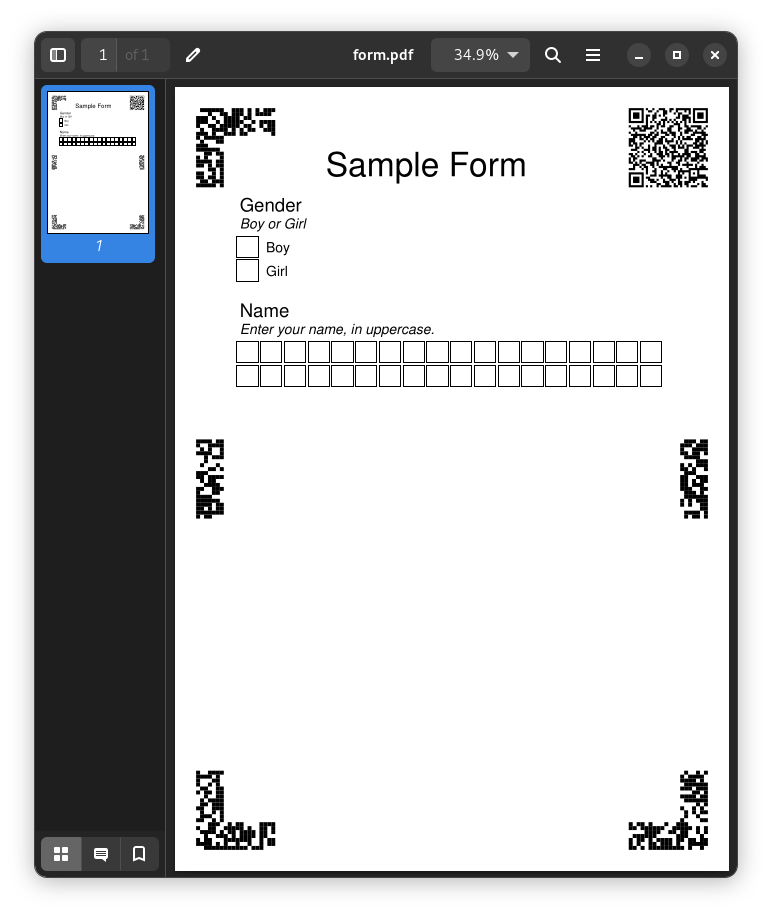
\includegraphics[width=20em]{images/screenshoots/sample_form.png}
    \caption{Sample form created with the SmartForms API}
    \label{fig:label}
\end{figure}

The features of the Pdf form are:
\begin{itemize}
    \item The questions, where users are prompted to either write an 'X', '*' or a similar symbol for multiple choice questions, and capital letters for regular questions.
    \item Lateral markers, forming a binary grid of small squares generated at random, which are added to maximize the number of features we can extract to match a scan / picture of the form with the original.
    \item The QR code (top right corner), playing a double role:
    \begin{itemize}
        \item Users can scan the form, which sends them to the webpage where they can fill the form online.
        \item The parsing software uses the QR code to extract the ID of the form, to know what it should look for.
    \end{itemize}
\end{itemize}

We can now add an answer directly from the API:

\definecolor{bg}{rgb}{0.95,0.95,0.95}
\begin{minted}[bgcolor=bg]{Shell}
teo@fedora ~> curl -X 'POST' \
                    'http://smartforms.ml:5000/api/entry/create' \
                    -H 'accept: application/json' \
                    -H 'Content-Type: application/json' \
                    -d '{
                "answerId": "",
                "formId": "af61ce94-db35-11ec-a6ed-dca6325bcf52",
                "authorEmail": "",
                "answers": [
                  "X ",
                  "Theodor Moroianu"
                ]
              }'
# the command returns the following JSON:
{
    "entryId":"entry-04896360-db67-11ec-a6ed-dca6325bcf52"
}
\end{minted}

We can also print the form, and fill it by hand. We can then pass to the inference API the following scan:

\begin{figure}[!h]
    \centering
    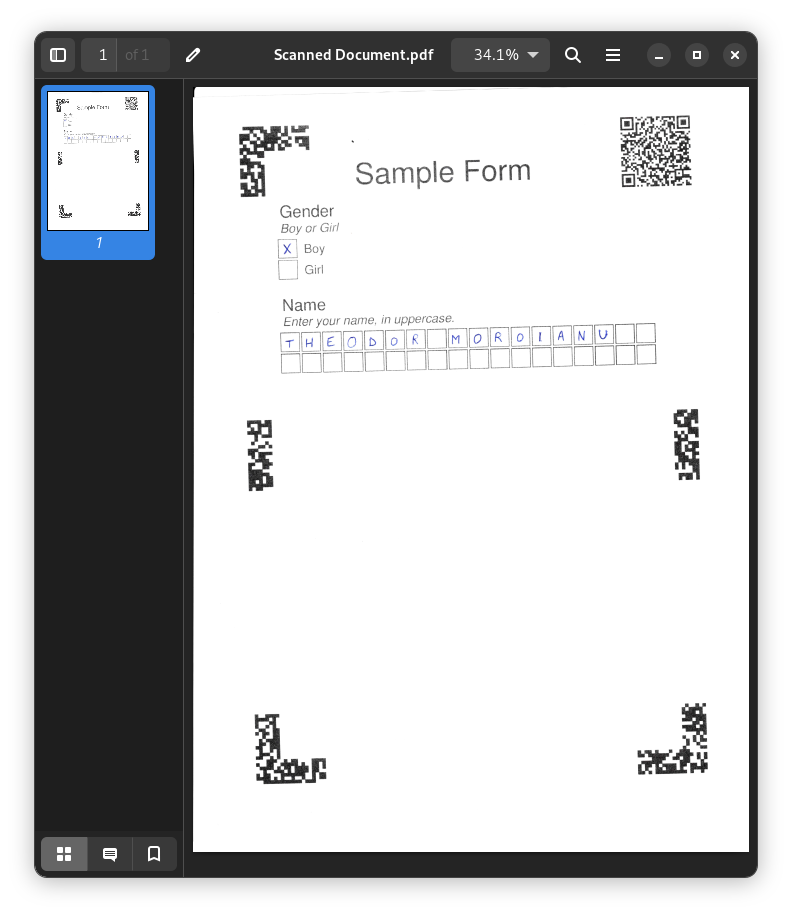
\includegraphics[width=30em]{images/screenshoots/sample_form_scan.png}
    \caption{Scan of a manually filled form}
    \label{fig:label}
\end{figure}


We then get back the following data:

\definecolor{bg}{rgb}{0.95,0.95,0.95}
\begin{minted}[bgcolor=bg]{Shell}
{
  "entries": [
    {
      "answerId": "entry-b7ef7ca8-db69-11ec-a510-704d7ba4fc42",
      "formId": "af61ce94-db35-11ec-a6ed-dca6325bcf52",
      "authorEmail": "theodor.moroianu@gmail.com",
      "answers": [
        "X ",
        "THEODOR MOROIANU                    "
      ],
      "creationDate": "2022-05-24T16:59:24.561788"
    }
  ],
  "errors": []
}
\end{minted}

SmartForms is able to:
\begin{enumerate}
    \item Correctly detect, from the QR code, the form present in the scan.
    \item Extract each individual answer square.
    \item Run the squares through an OCR neural network, to predict the most plausible character.
    \item Add the answers to the database and return them to the users.
\end{enumerate}

It should be noted that the process is not flawless, and is discussed in more details in the Form Parsing section.
\\


We can now query the API to retrieve our two entries:

\definecolor{bg}{rgb}{0.95,0.95,0.95}
\begin{minted}[bgcolor=bg]{Shell}
teo@fedora ~> curl -X 'POST' \
                    'http://smartforms.ml:5000/api/entry/view-form-entries' \
                    -H 'accept: application/json' \
                    -H 'Content-Type: application/json' \
                    -d '{
                "formId": "af61ce94-db35-11ec-a6ed-dca6325bcf52",
                "offset": 0,
                "count": 2
              }' | python -m json.tool
  % Total    % Received % Xferd  Average Speed   Time    Time     Time  Current
                                 Dload  Upload   Total   Spent    Left  Speed
100   568  100   485  100    83   1473    252 --:--:-- --:--:-- --:--:--  1726
{
    "entries": [
        {
            "answerId": "entry-04896360-db67-11ec-a6ed-dca6325bcf52",
            "formId": "af61ce94-db35-11ec-a6ed-dca6325bcf52",
            "authorEmail": "theodor.moroianu@gmail.com",
            "answers": [
                "X ",
                "Theodor Moroianu"
            ],
            "creationDate": "2022-05-24T13:40:04.586000"
        },
        {
            "answerId": "entry-b7ef7ca8-db69-11ec-a510-704d7ba4fc42",
            "formId": "af61ce94-db35-11ec-a6ed-dca6325bcf52",
            "authorEmail": "theodor.moroianu@gmail.com",
            "answers": [
                "X ",
                "THEDDOR MOROIANU                    "
            ],
            "creationDate": "2022-05-24T16:59:24.561000"
        }
    ],
    "totalFormsCount": 2
}
\end{minted}

We can, in a similar fashion, edit / delete answers and forms.


% dau mai multe detalii despre cum 
% functioneaza baza de date mongodb
\chapter{Storage System}

\section{Choosing MongoDB}
We explored multiple database systems for our application. For choosing the most suited one, we made a list of requirements:

\begin{itemize}
    \item We need an easy to set-up, efficient system we can install on relatively small devices.
    \item We need a system well integrated within the \textit{Python} ecosystem.
    \item We need a system able to run both locally and in the cloud, to accommodate the different working scenarios of \textit{SmartForms}.
\end{itemize}

On the other hand, we do not need:
\begin{itemize}
    \item A system able to process massive amounts of data, as the database is mainly used for storing form descriptions and form answers.
    \item A system able to perform complex \code{joins} or similar operations typically done with the help of a \textit{DML} (Data Manipulation Language). 
\end{itemize}

The database system we decided to use within \textit{SmartForms} is \textit{MongoDB}, a document-based, No-SQL database storing data as \textit{JSON} objects.


\begin{figure}[!h]
    \centering
    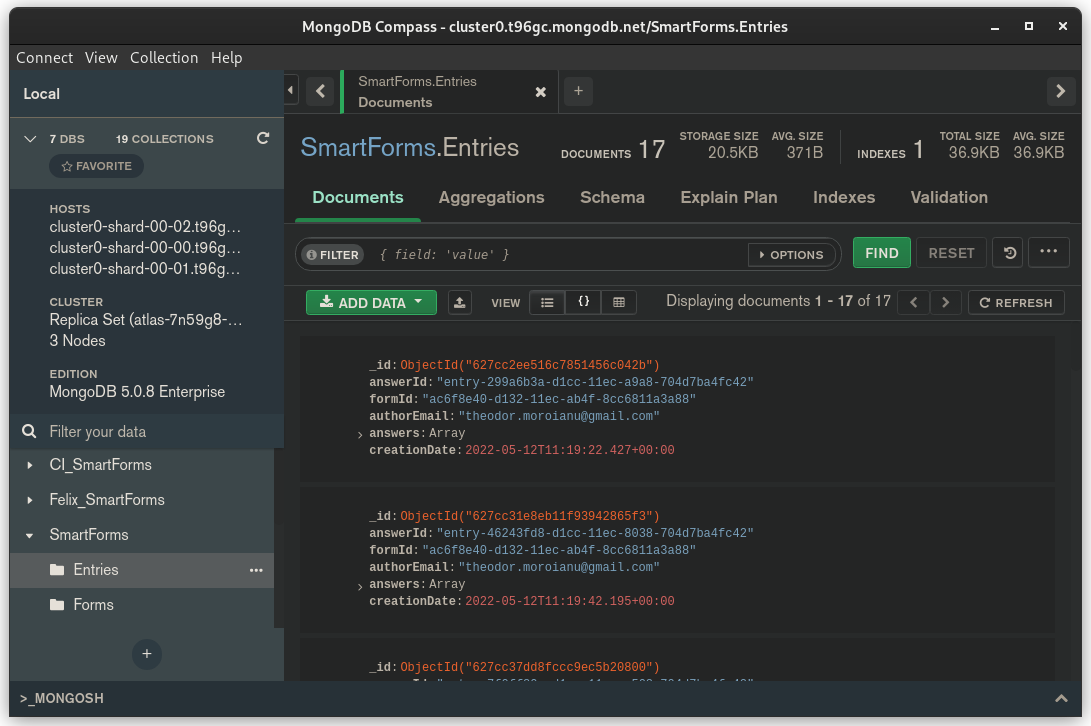
\includegraphics[width=35em]{images/screenshoots/mongo-compas.png}
    \caption{Compass -- the official MongoDB viewer}
    \label{fig:label}
\end{figure}

The connection to \textit{MongoDB} is done in the \code{database} module. The URI, username and password are specified with the help of the \code{.env} secrets file, which in the current configuration connects \textit{SmartForms} to a database stored on the cloud:

\definecolor{bg}{rgb}{0.95,0.95,0.95}
\begin{minted}[bgcolor=bg]{Shell}
# Connect to Mongo Cloud
MONGO_USER='smart-forms-user'
MONGO_PASSWORD='*********'
MONGO_CLUSTER='cluster0.t96gc.mongodb.net'
MONGO_DB_NAME='SmartForms'
\end{minted}

\section{Information Stored in MongoDB}

MongoDB databases, contain multiple collections storing entries, similar to SQL databases containing tables storing rows.

We set-up multiple databases:
\begin{itemize}
    \item A database used for production.
    \item Another database used for the \textit{CI/CD} pipelines.
    \item Databases used for local development and testing without disturbing the other environments. 
\end{itemize}

Databases store the information used by \textit{SmartForms}. As forms and answers requested by the users are unpredictable, and \textit{SmartForms} is built to be able to run on relatively low-end devices, locally caching data for lower latency didn't make sense. As such, any CRUD (Create, Read, Update or Delete) operations performed on forms, answers or users are directly committed to the database.


\begin{figure}[!h]
    \centering
    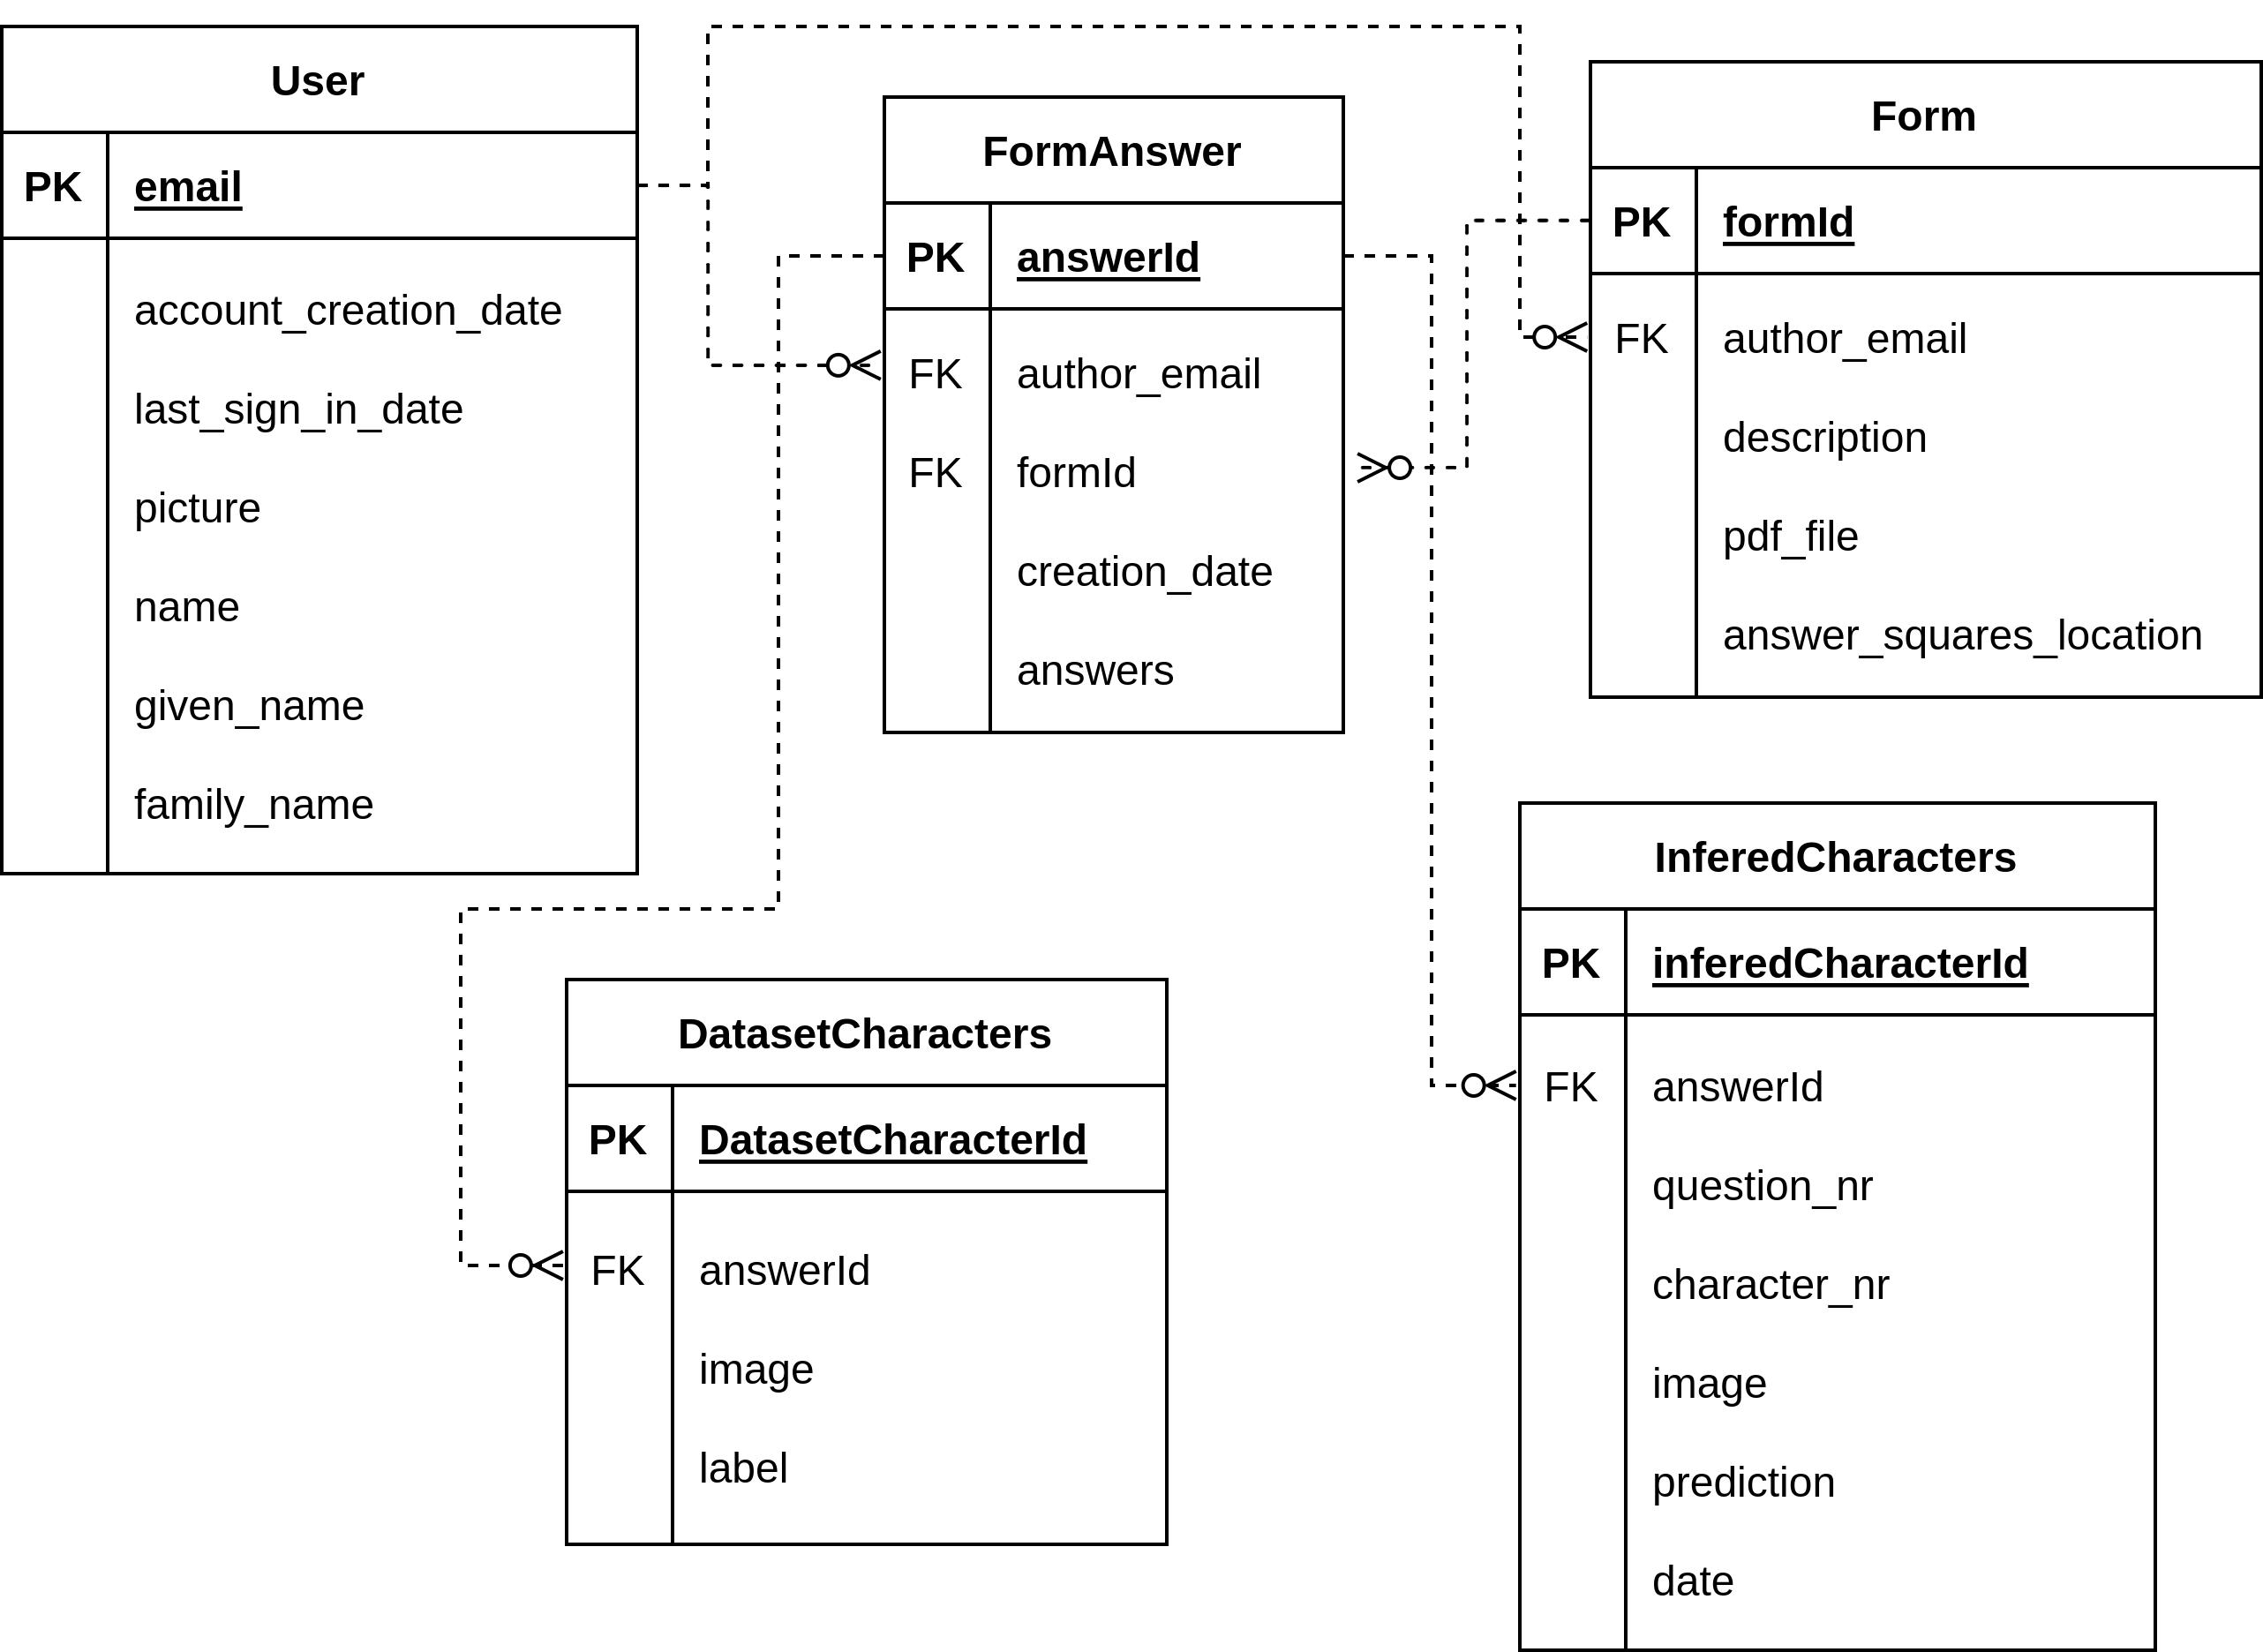
\includegraphics[width=35em]{images/diagrams/ER_diagram.png}
    \caption{Diagram of the MongoDB Database}
    \label{fig:label}
\end{figure}


The database stores:
\begin{itemize}
    \item The registered users. The information saved is the name, email, date of registration and last sign-in, and an URL to a profile picture if available. To be compliant with data-protection laws like the GDPR, we only use the personal data for authentication purposes, and delete all of an user's records when he/she deletes his/her account.
    \item The created forms -- for which we store the description, owner, creation date and the internal representation of the corresponding PDF document.
    \item The answers, both added directly with the API or uploaded as a scan or a picture.
    \item Images of the squares extracted from pictures and scans.
    \item A dataset of labeled characters which can be used for improving the OCR neural network.
\end{itemize}


The last two collection -- namely the \code{DatasetCharacters} and the \code{InferedCharacters} are used for automatically labeling characters, thus generating a dataset we can then use for fine-tuning the OCR neural network. A more detailed explanation of the process is done in the \textit{Form Parsing} section.


% Arat cum generez pdf-ul, si cum
% salvez un pdf generat.
\chapter{Pdf Forms Creation}

\section{Objective and Constraints}

The primary objective when generating a \textit{PDF} form is getting a concise, easy to understand and professional looking document, which can then be efficiently parsed and digitized.

The main contraints and details we have to consider are:
\begin{itemize}
    \item While in most usecases users want to print their forms on \textit{A4} paper, we should also make forms printable on smaller or larger paper.
    \item We want to allow both scans and pictures, made by a wide range of devices, in which brightness, color saturation and contrast differ.
    \item Modern smartphone cameras, because of the shrinkage of the size of their optical instruments, add slight distortions to the pictures (lines become curves). As each camera is different, fixing the distortions ourselves is not feasable.
    \item Even though most printers advertise the ability to print edge-to-edge, most modern printers aren't able to print anything too close to the edge of the paper.
    \item As most office printers only print in black and white for efficiency reasons, we shouldn't include color in our documents.
    \item People have extremely diverse styles of handwriting, which makes parsing cursive text with high accuracy difficult, even with modern technology.
    \item Forms can have varying lengths, from a simple question to multiple pages.
\end{itemize}

\section{Layout of a Pdf Form}

To not violate any of the constraints mentioned above, we embedd multiple components in the documents.

\subsection{Questions}

Questions are the most obvious element of the forms. They are made out of a question title -- or simply speaking the question, a question subtitle (or explanation) which is optional, and input zones depending on the type of question.

\begin{figure}[!h]
    \centering
    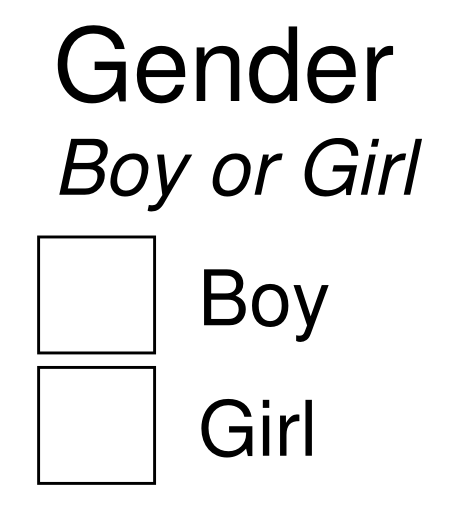
\includegraphics[width=8em]{images/screenshoots/sample-multiple-choice-question.png}
    \caption{Sample multiple-choice question}
    \label{fig:label}
\end{figure}

If the question is a multiple choice question, where the user has to select a subset of the given possibilities (e.g. "Boy" or "Girl"), the each option is printed on a different line, with a square the user can tick to select the question.


\begin{figure}[!h]
    \centering
    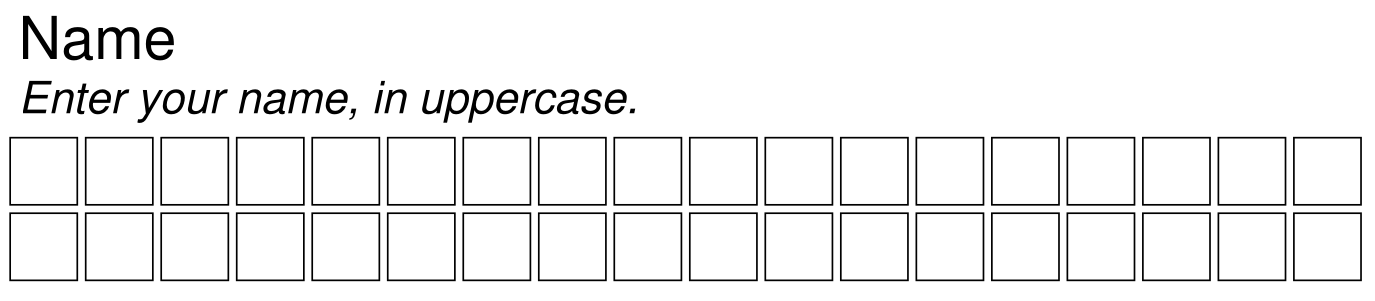
\includegraphics[width=40em]{images/screenshoots/sample-text-question.png}
    \caption{Sample text question}
    \label{fig:label}
\end{figure}

If the question is a text question, then a user-specified number of squares are printed. People filling the form can then write one letter per square.

The main advantages of this approach are:
\begin{itemize}
    \item Multiple-choice and text questions can be processed similarly, as we simply want to check if boxes from the multiple choice questions contain an 'X', 'V', '*' or similar marker.
    \item This format is writing-style agnostic, as users are forced to write each letter to a specific location in a specific format.
    \item The forms are easy to understand and fill-in.
\end{itemize}

Note that the exact location of each square is saved in the database, to allow later pinpointing of the exact pixels of each character.

\subsection{Markers}

Lateral matching helpers, or markers, are irregular patterns we print on the corners.

\begin{figure}[!h]
    \centering
    
\includegraphics[width=10em]{images/screenshoots/top-left-marker.png}
    \caption{Top left marker}
    \label{fig:label}
\end{figure}

Similar shapes are often printed on objects that robots or software agents need to be able to identify, due to their vast number of descriptors. \textit{SmartForms} uses a \textit{ORB} feature extractor\cite{rublee2011orb}, which relies on intensity differences between adjacent pixels.

With the help of the \textit{ORB} feature extractor, we can then match extracted features of the blank Pdf document with a picture or scan, to get an accurate rectangular representation of the scanned image.

\subsection{QR Code}

QR codes (shorthand for Quick Response codes) are visual machine barcodes. QR codes are machine-readable, use the Reed–Solomon error correction algorithm\cite{wicker1999reed}, and can store arbitrary data, from Wi-Fi details to contacts or simple text.

\begin{figure}[!h]
    \centering
    
\includegraphics[width=13em]{images/screenshoots/sample-qr-code.png}
    \caption{QR code with content "\textit{https://smartforms.ml/view-form/af61...}"}
    \label{fig:label}
\end{figure}

We use QR codes for multiple reasons:
\begin{itemize}
    \item Due to their apparent randomness, they also help the feature extraction of the matching process.
    \item They offer an easy-to-follow link to the \textit{SmartForms} website, which users can open to fill the form online.
    \item It allows the matching software to extract the form ID, to figure out which form is being parsed.
\end{itemize}

\subsection{Preview Notice}

Users tend to commit their work more often than is strictly required: people writing documents save them every few minutes, developers writing code compile it to check for mistakes, and, to no surprise, people generating forms tend to preview intermediate results.

As such, adding each intermediate result to the database doesn't make much sense. On the other hand, users have to easily see if a form is valid or not. This is why, on forms which are only made for preview, we print an additional "\textit{PREVIEW}" banner.


\begin{figure}[!h]
    \centering
    \fbox{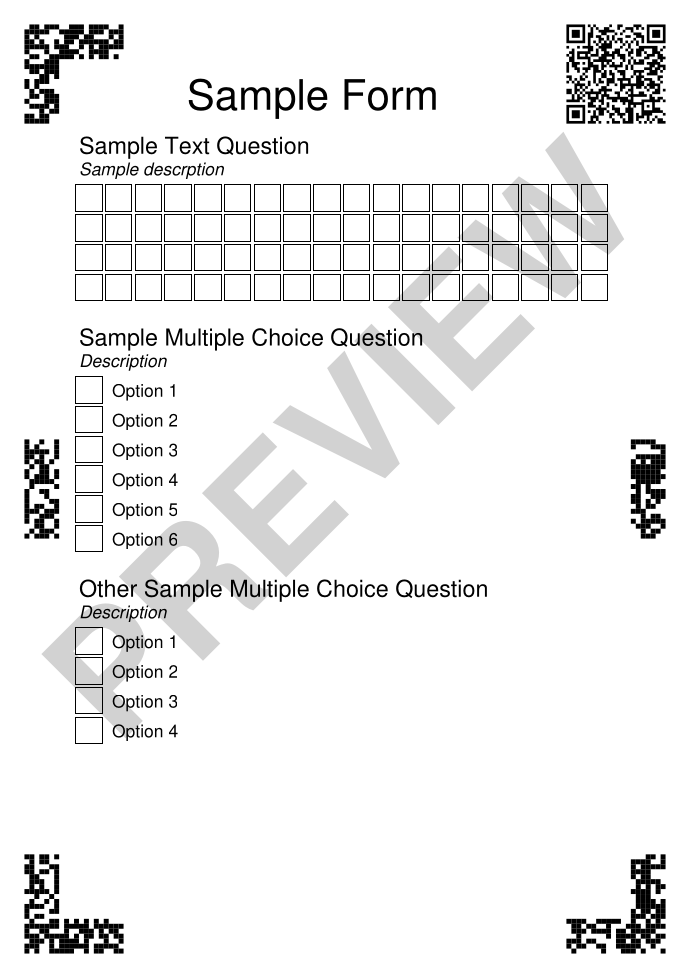
\includegraphics[width=30em]{images/screenshoots/sample-preview-form.png}}
    \caption{Form with "\textit{PREVIEW}" banner.}
    \label{fig:label}
\end{figure}

\subsection{Multi-page Support}

If the form has many questions, then the Pdf document might spread among multiple pages. In such situations, each page gets a unique ID encoded within the QR code, to allow the parsing pipeline to order them accordingly.

The lateral markers and the optional preview notice are present on all the pages.



% Arat cum fac matchingul si ocr-ul.
% tot aici vorbesc despre CNN
\chapter{Form Parsing}

\section{How Data is Loaded}

The API relies on the \code{multipart/form-data}\cite{masinter1998rfc2388} format to receive reliably larger files than what is usually permitted over the \textit{HTTP} protocol.

To facilitate the uploading of filled forms, we accept:
\begin{itemize}
    \item A list of images, in any of the standard image formats (\code{.jpeg}, \code{.png}, \code{.webp} etc).
    \item A list of PDF documents.
    \item A \textit{Zip} archive, the content of which is processed recursively.
\end{itemize}

Due to the high flexibility and permissive formats supported by \textit{SmartForms}, virtually any structured folder of forms can be zipped, uploaded and parsed.

Once the backend receives the files, it automatically deflates all zip files, and:
\begin{enumerate}
    \item Considers each PDF as a folder, whose content are the pages of the document (each page is considered as a single picture).
    \item Splits all the images into groups, according to their containing folder.
    \item Parses each group as a single form.
\end{enumerate}

\section{Finding the Template}

Given a set of images (obtained directly from the user, from a zip file or extracted from a page of a PDF document), the backend has to figure out which form is being parsed.

To do this quickly and reliably, we look for the QR code inserted on each document. Finding the QR code is itself a challenge, as most libraries used for scanning QR codes (like the ones used on mobile phones) expect a close-up picture of the code. However, because we can't know the orientation, size or location of the form in the received picture, we can't reliably determine the exact location of the QR code.

For solving this issue, we use \code{Zbar}, an open-source bar reading library written in \textit{C}. While the application isn't written in \textit{Python} for compatibility and performance reasons, the \code{pyzbar} package provides \textit{Python} bindings we can use.

\textit{Zbar} is highly optimized for real-time barcodes and QR codes scanning, and can be also used from a terminal. By passing it the form we created above we get:


\definecolor{bg}{rgb}{0.95,0.95,0.95}
\begin{minted}[bgcolor=bg]{Shell}
teo@fedora ~> zbarimg Scanned\ Document.pdf 
QR-Code:
https://smartforms.ml/view-form/af61ce94-db35-11ec-a6ed-dca6325bcf52

scanned 1 barcode symbols from 1 images in 0.02 seconds
\end{minted}

Please note that the text extracted by \textit{Zbar} is not the actual ID of the form, but rather an URL to the \textit{SmartForms} website, where, depending on permissions, users may fill the form online. To extract the real ID, we simply have to remove the "\textit{https://smartforms.ml/view-form/}" prefix. \textit{Pyzbar} operates in a similar way, but can be called from within \textit{Python} code.

With the form ID, we can query the \textit{MongoDB} database to extract all the required details about the form.

\section{Applying Graysclale and Binary Threshold}

\begin{figure}[!h]
\hfill
\subfigure[Original]{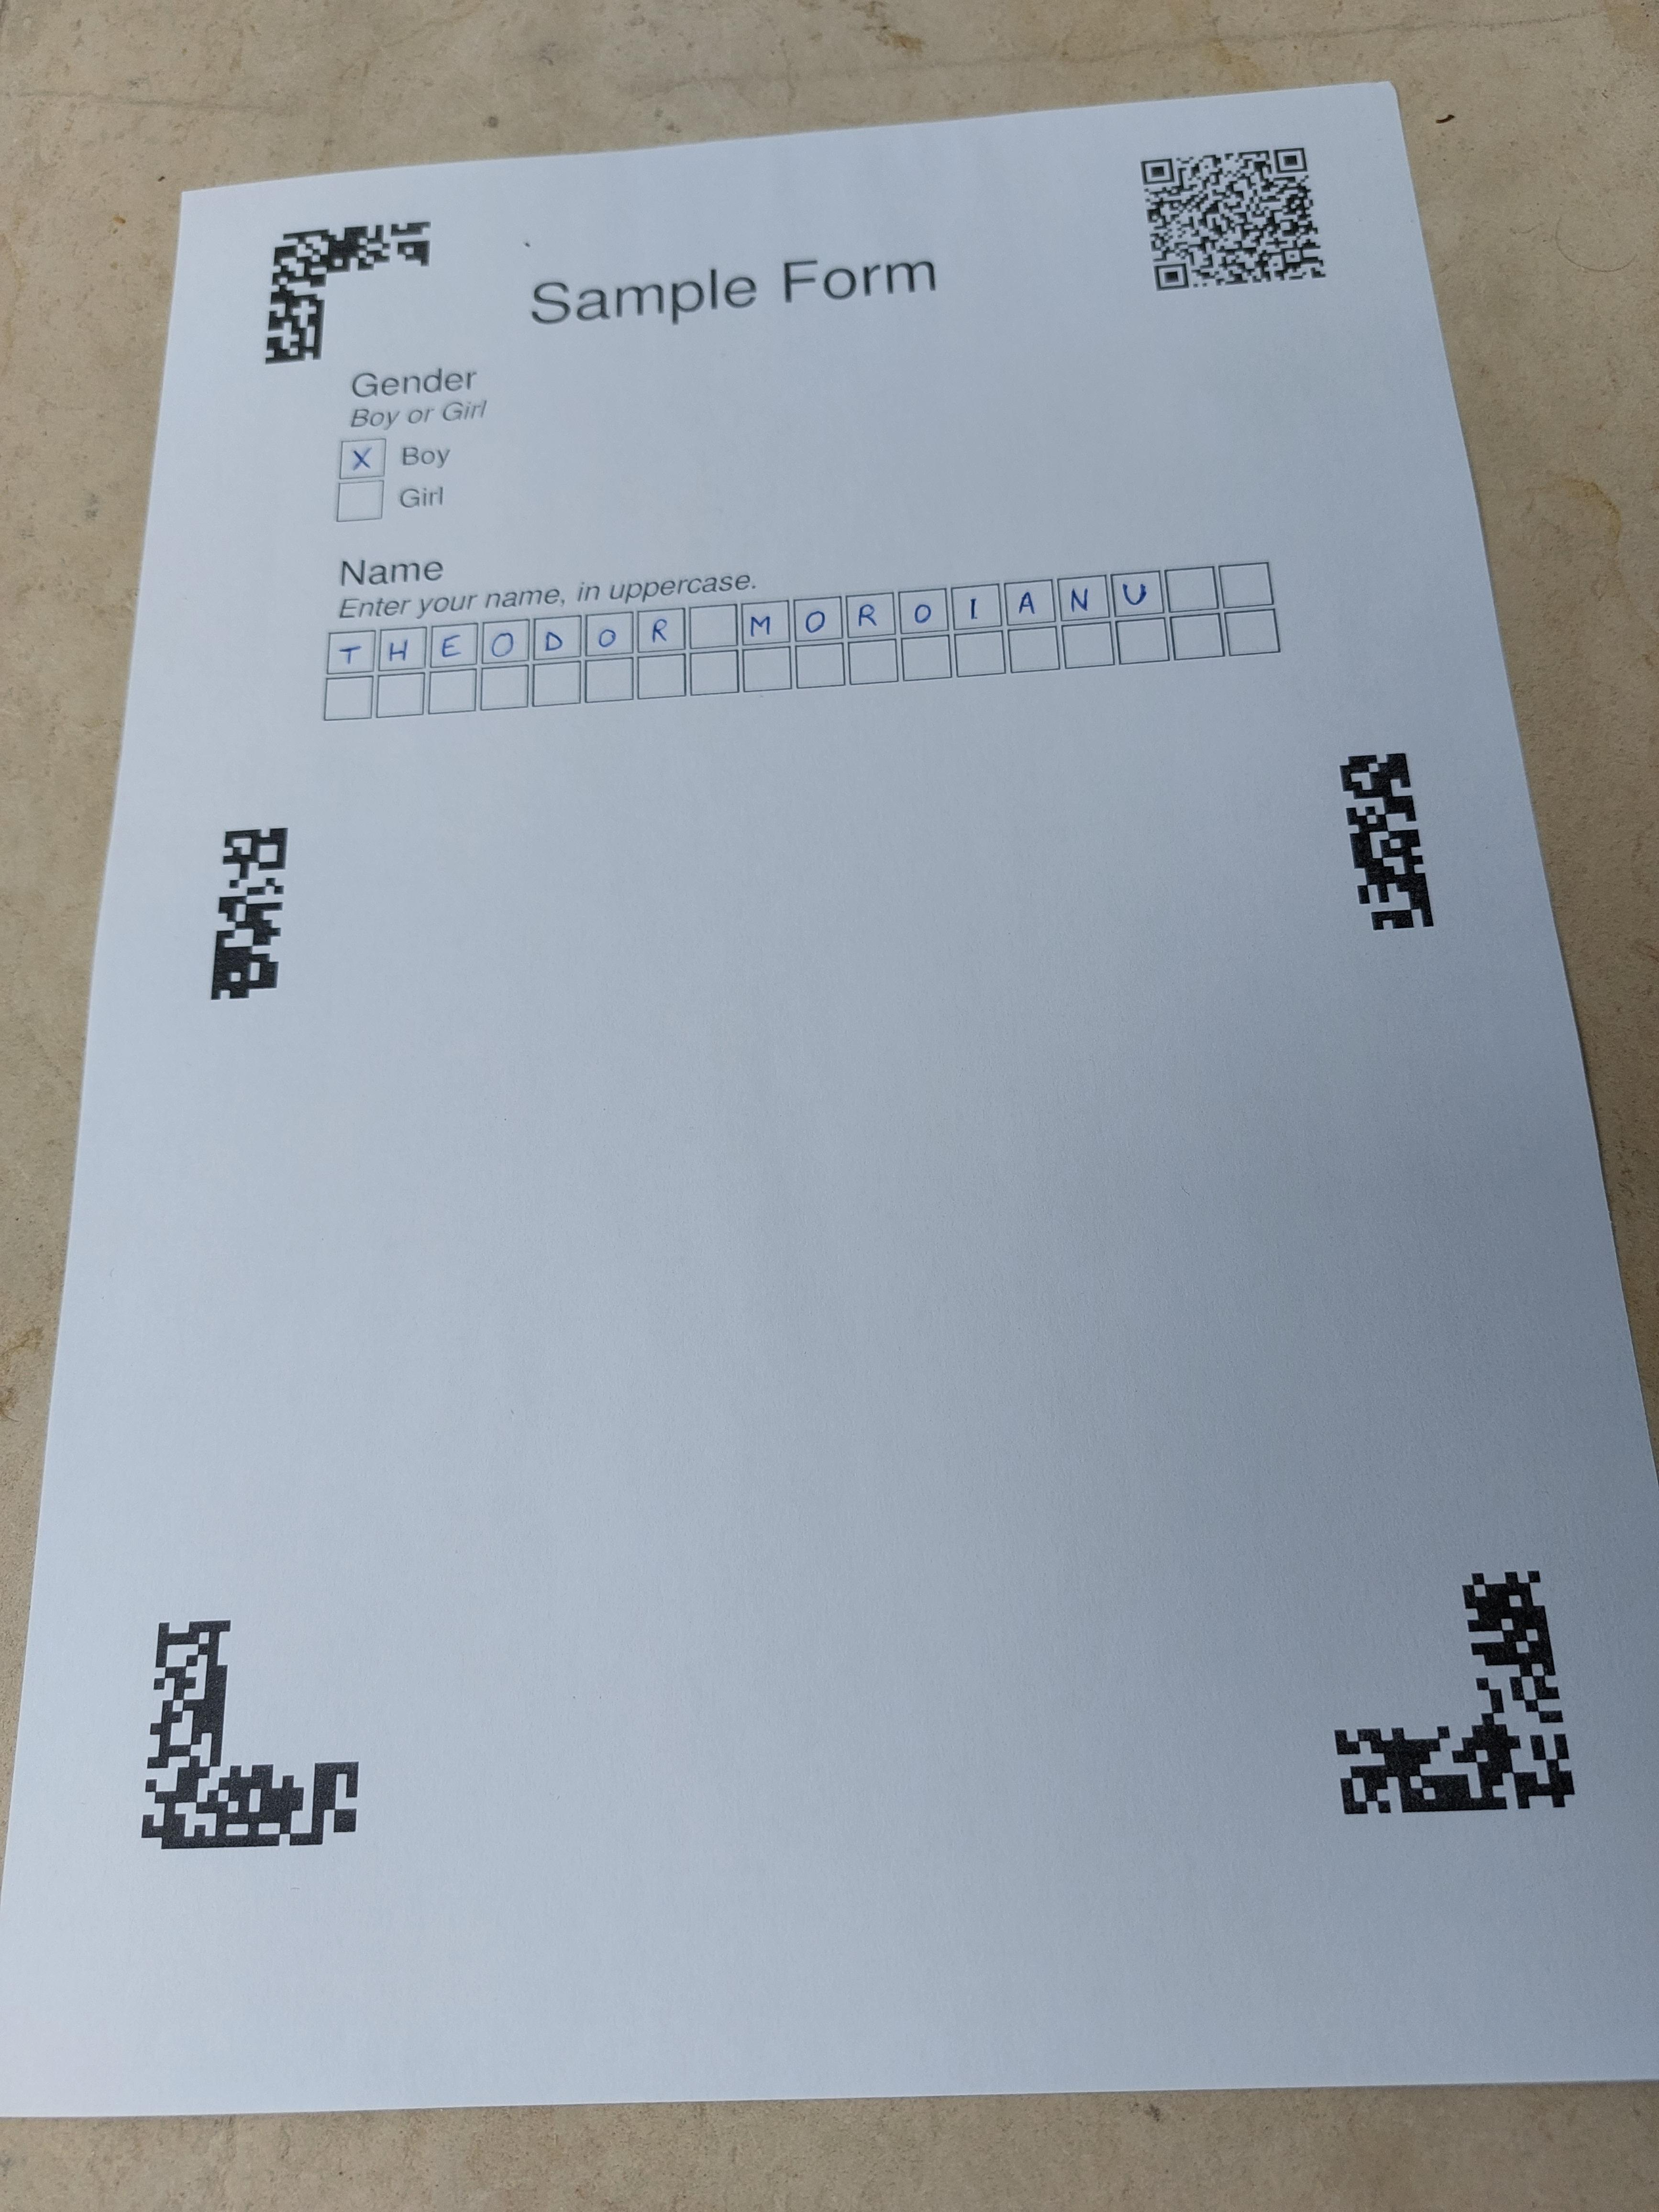
\includegraphics[width=6cm]{images/graphs/original_image.jpg}}
% \hfill
\subfigure[Processed]{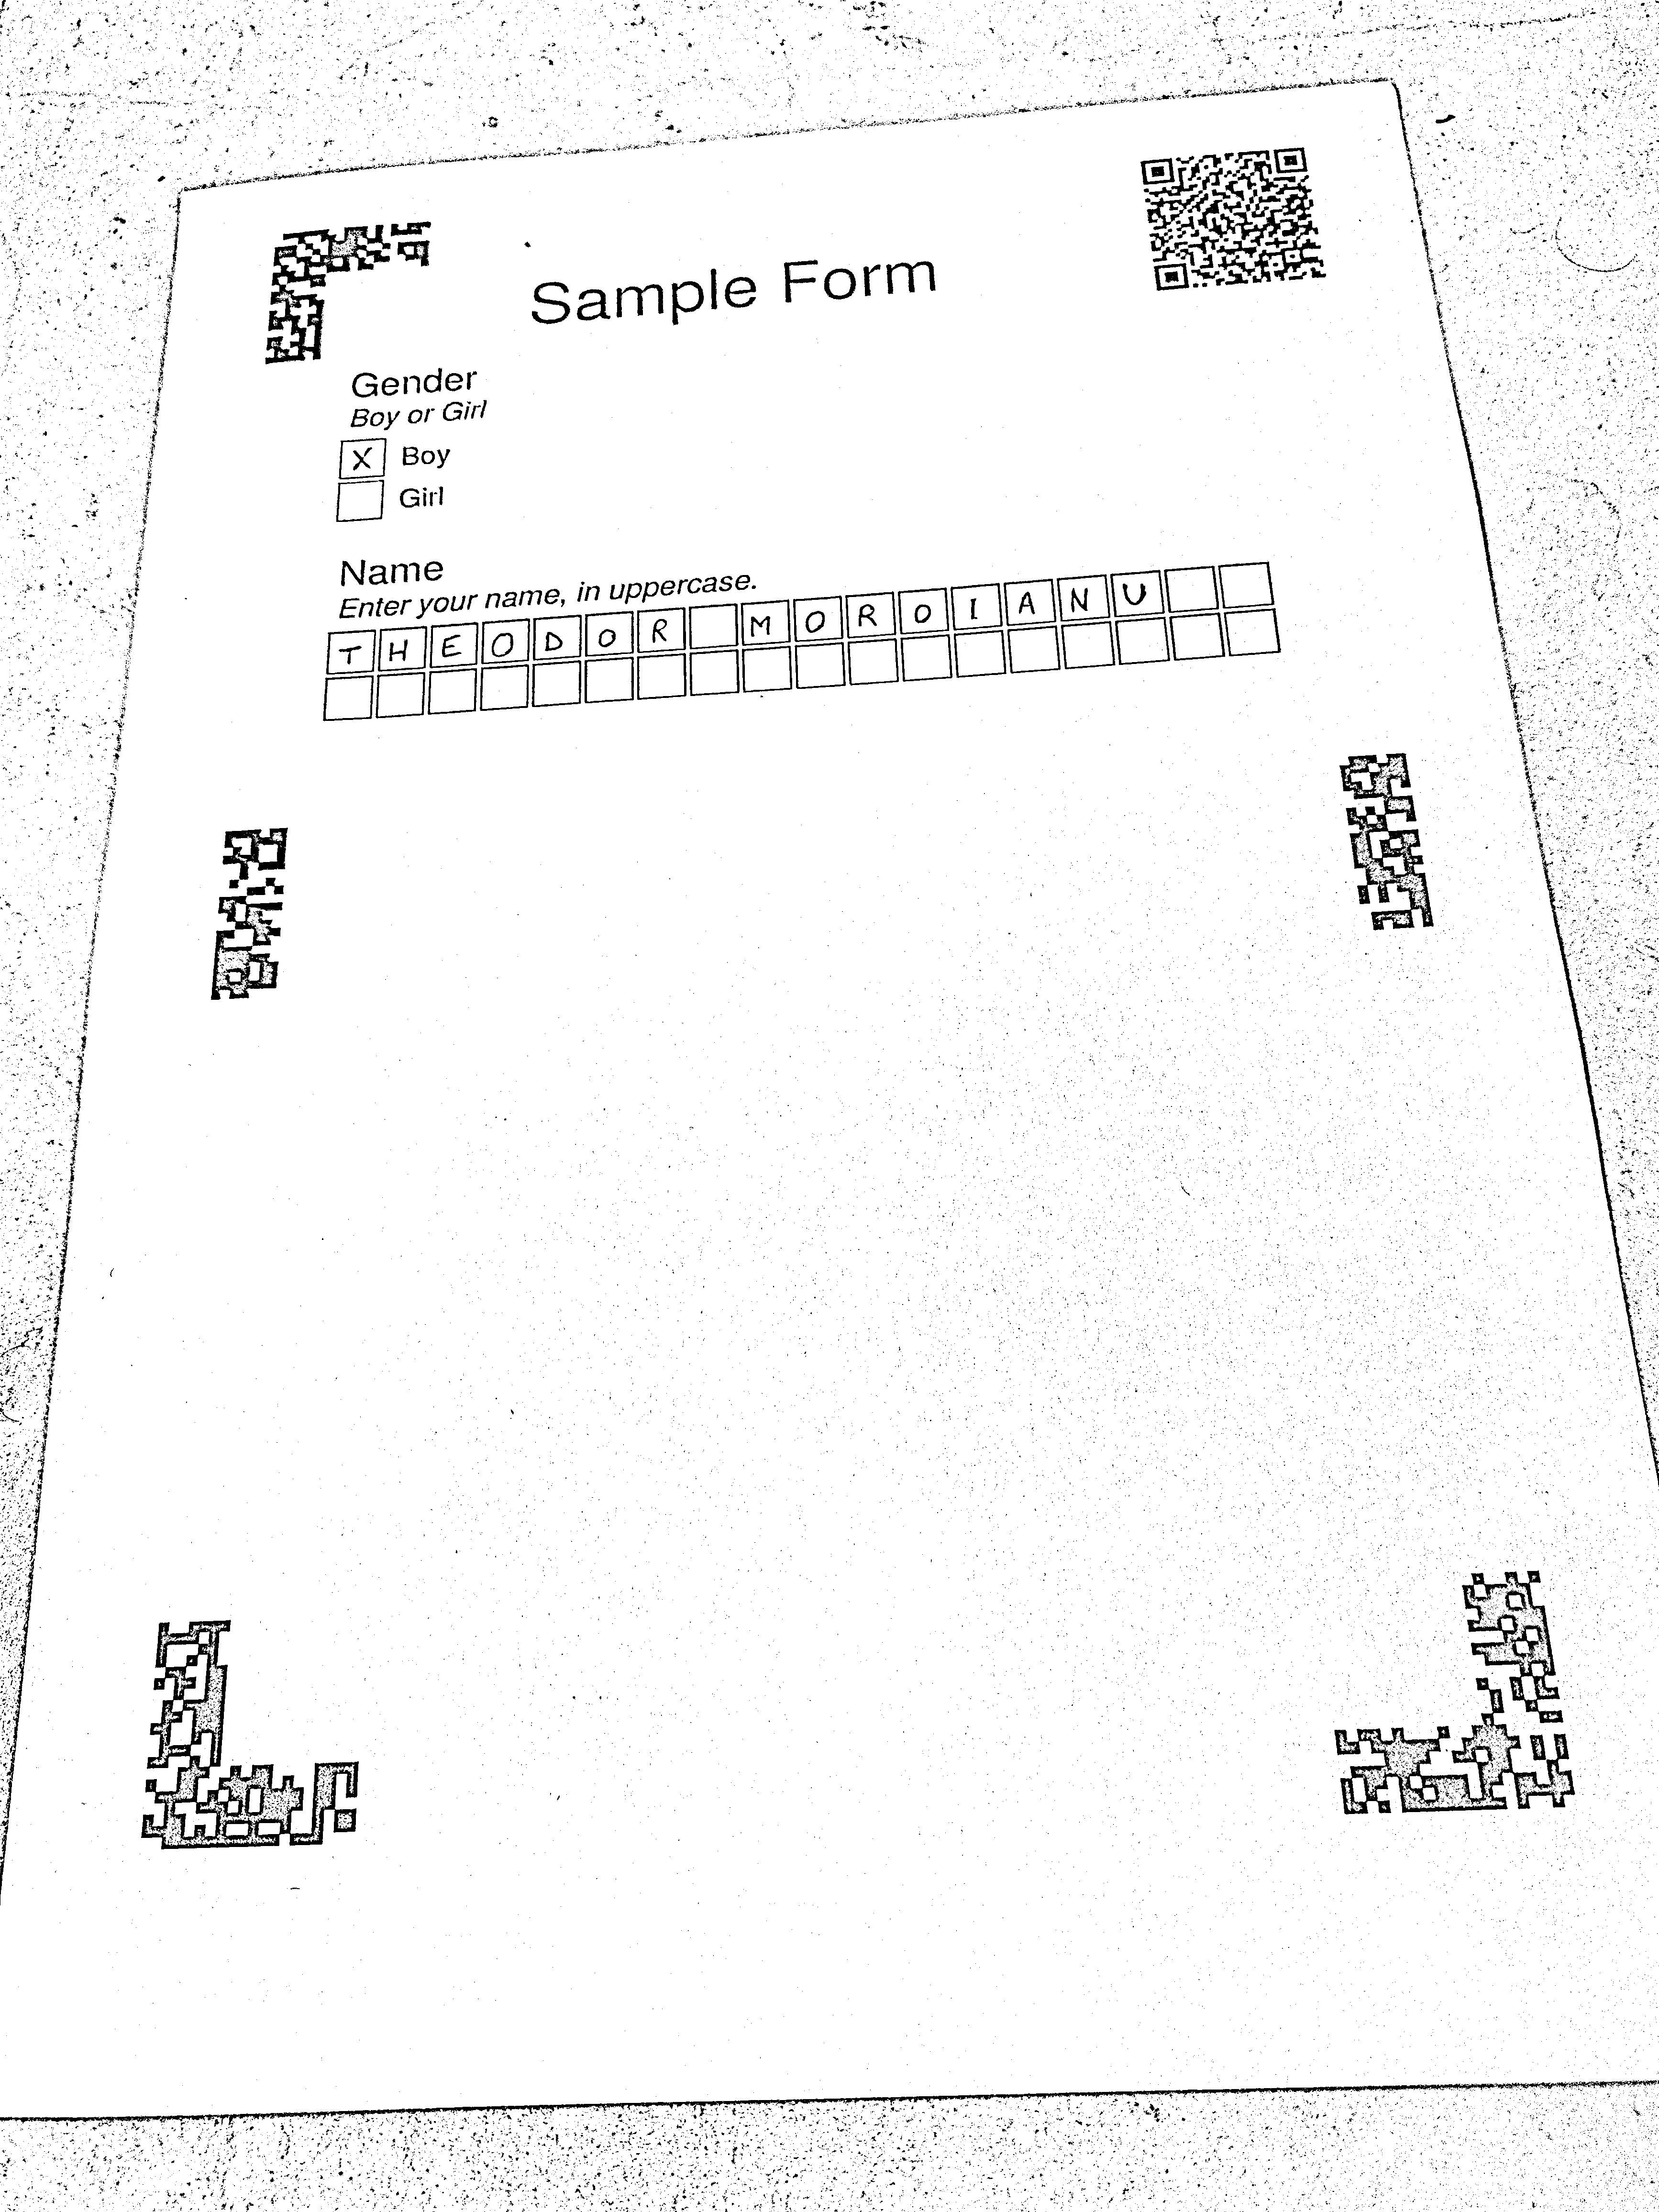
\includegraphics[width=6cm]{images/graphs/parser_processed_image.jpg}}
\hfill
\caption{Picture converted to binary}
\label{original-vs-processed-image}
\end{figure}

Most image processing algorithms rely on grayscale or binary images. As such, we first have to convert our colored image to grayscale, and then apply a binary threshold.

To convert an image to grayscale, we can independently transform each pixel from a \code{RGB} value to a single channel. \textit{OpenCV}, the machine vision framework we are using, converts an image to grayscale using the following formula\cite{opencv-color-convention}:

$$Y = 0.299*R+0.587*G+0.114*B$$

Our first step is converting a picture or scan of our form into grayscale. Figure \ref{original-vs-processed-image} (a) shows what such a picture might look like. However, even with the image in grayscale we cannot simply apply a standard binary threshold, due to possible differences in brightness.

 \begin{figure}[!h]
  \centering
  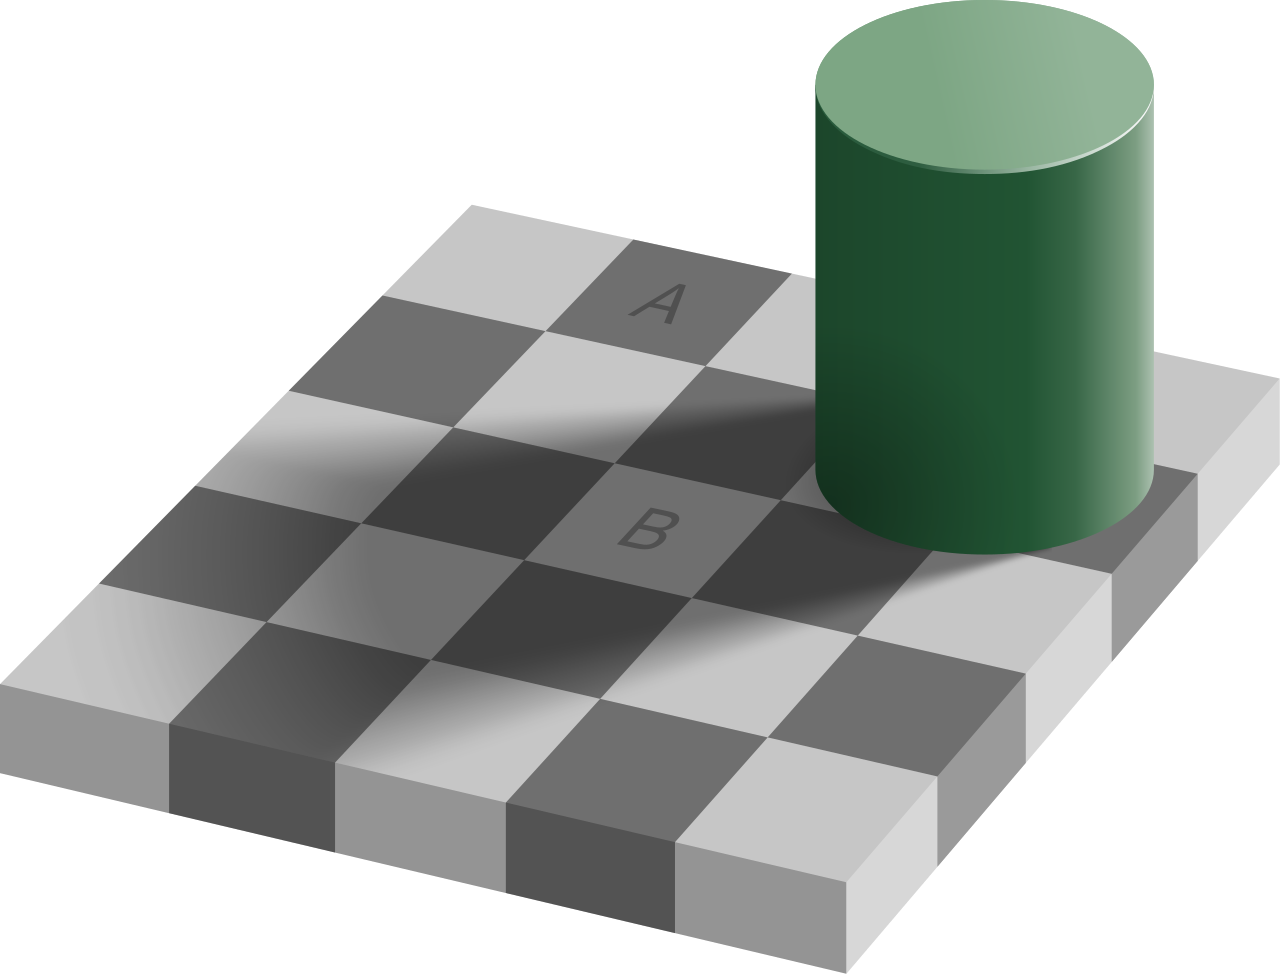
\includegraphics[width=20em]{images/other/Checker_shadow_illusion.svg.png}
  \caption{Checker Shadow Illusion\cite{checker-illusion}}
  \label{checker-illusion}
\end{figure}

As ilustrated in Figure \ref{checker-illusion}, where squares marked with \textbf{A} and \textbf{B} seem different even though the color is the same, separating dark and light regions is not a trivial task, if we want to take into account lighing and brightness. Similarly, applying a binary threshold considering pixel intensities larger than a fixed $K$ black and intensities smaller than $K$ white will lead to misclassified pixels, where darker empty regions of the form might be classified as black, and similarly lighter text or graphics of the form might get classified as white.

To convert our grayscale image to binary, we use an adaptive thresholding technique\cite{opencv-image-threshold}, which for each pixels determines, based on a small region around it, if it should be black or white. Applying such an algorithm over our grayscale image gives us an image similar to Figure \ref{original-vs-processed-image} (b).


%Ca in figura \ref{etichetaTT}

\section{Changing Image Perspective}

% \begin{figure}[!h]%
%     \centering
%     \subfloat[\centering label 1]{{
%     \rotatebox[origin=c]{90}{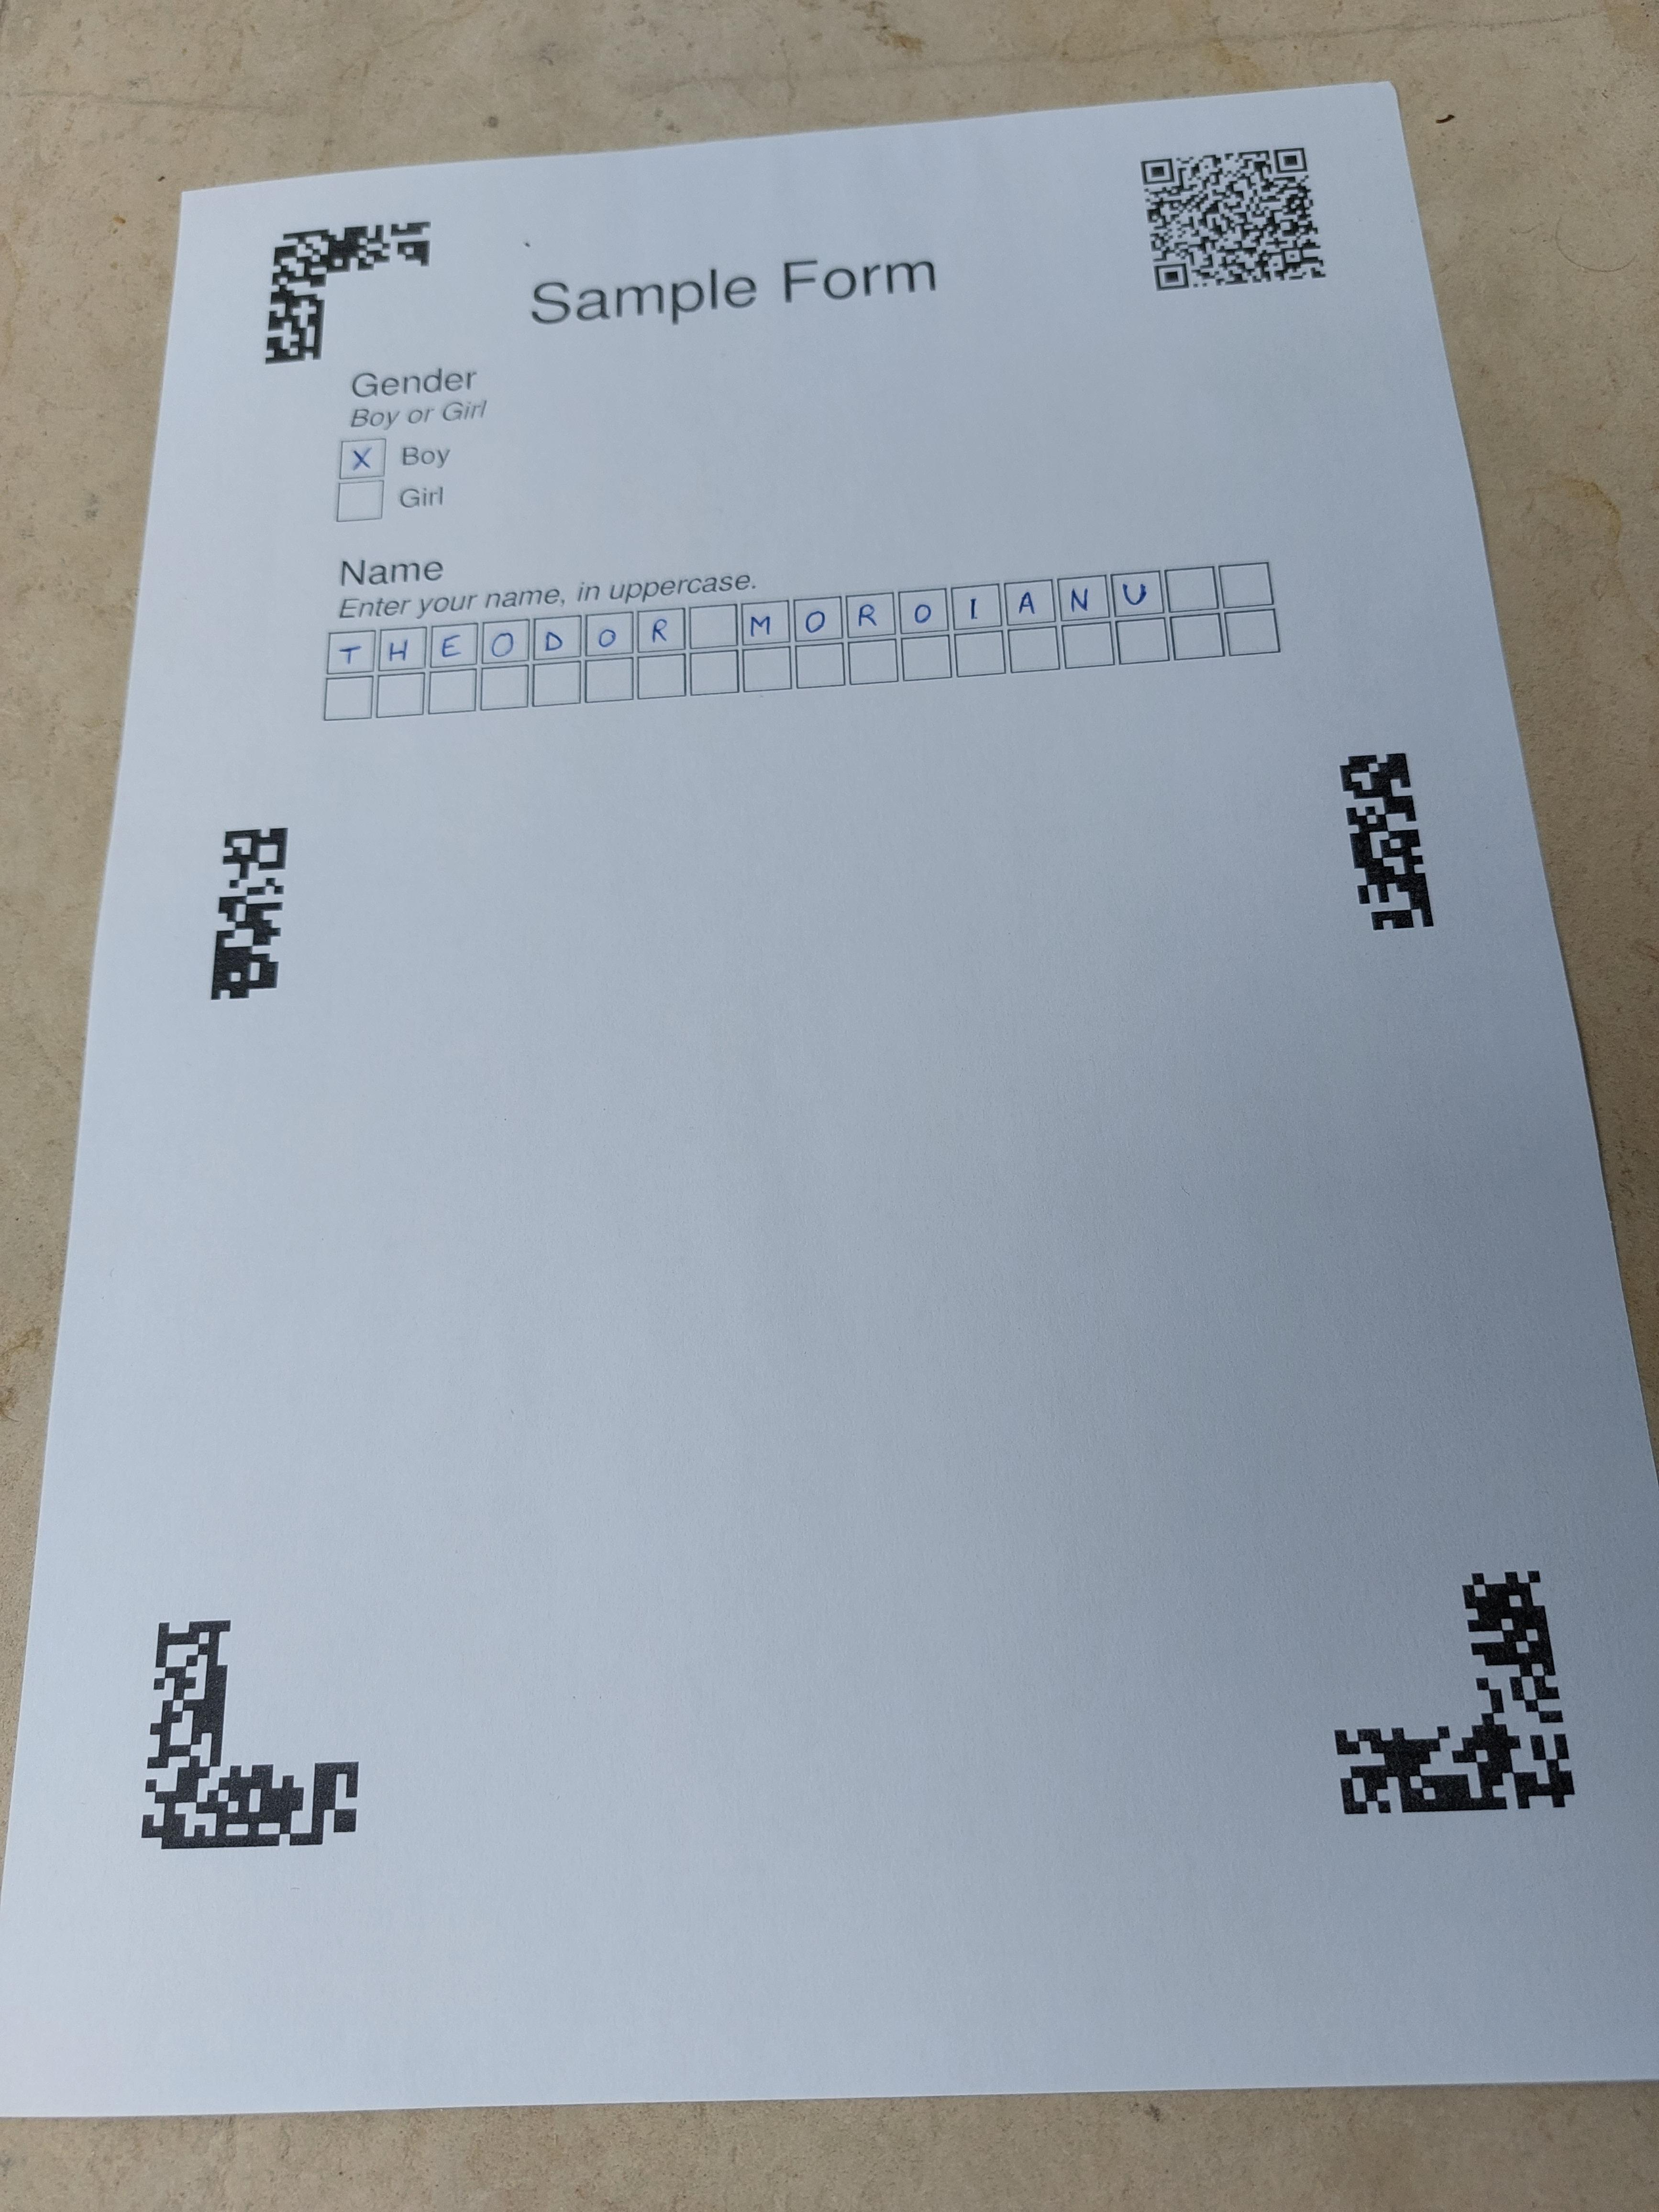
\includegraphics[width=5cm]{images/graphs/original_image.jpg}} }}%
%     \qquad
%     \subfloat[\centering label 2]{{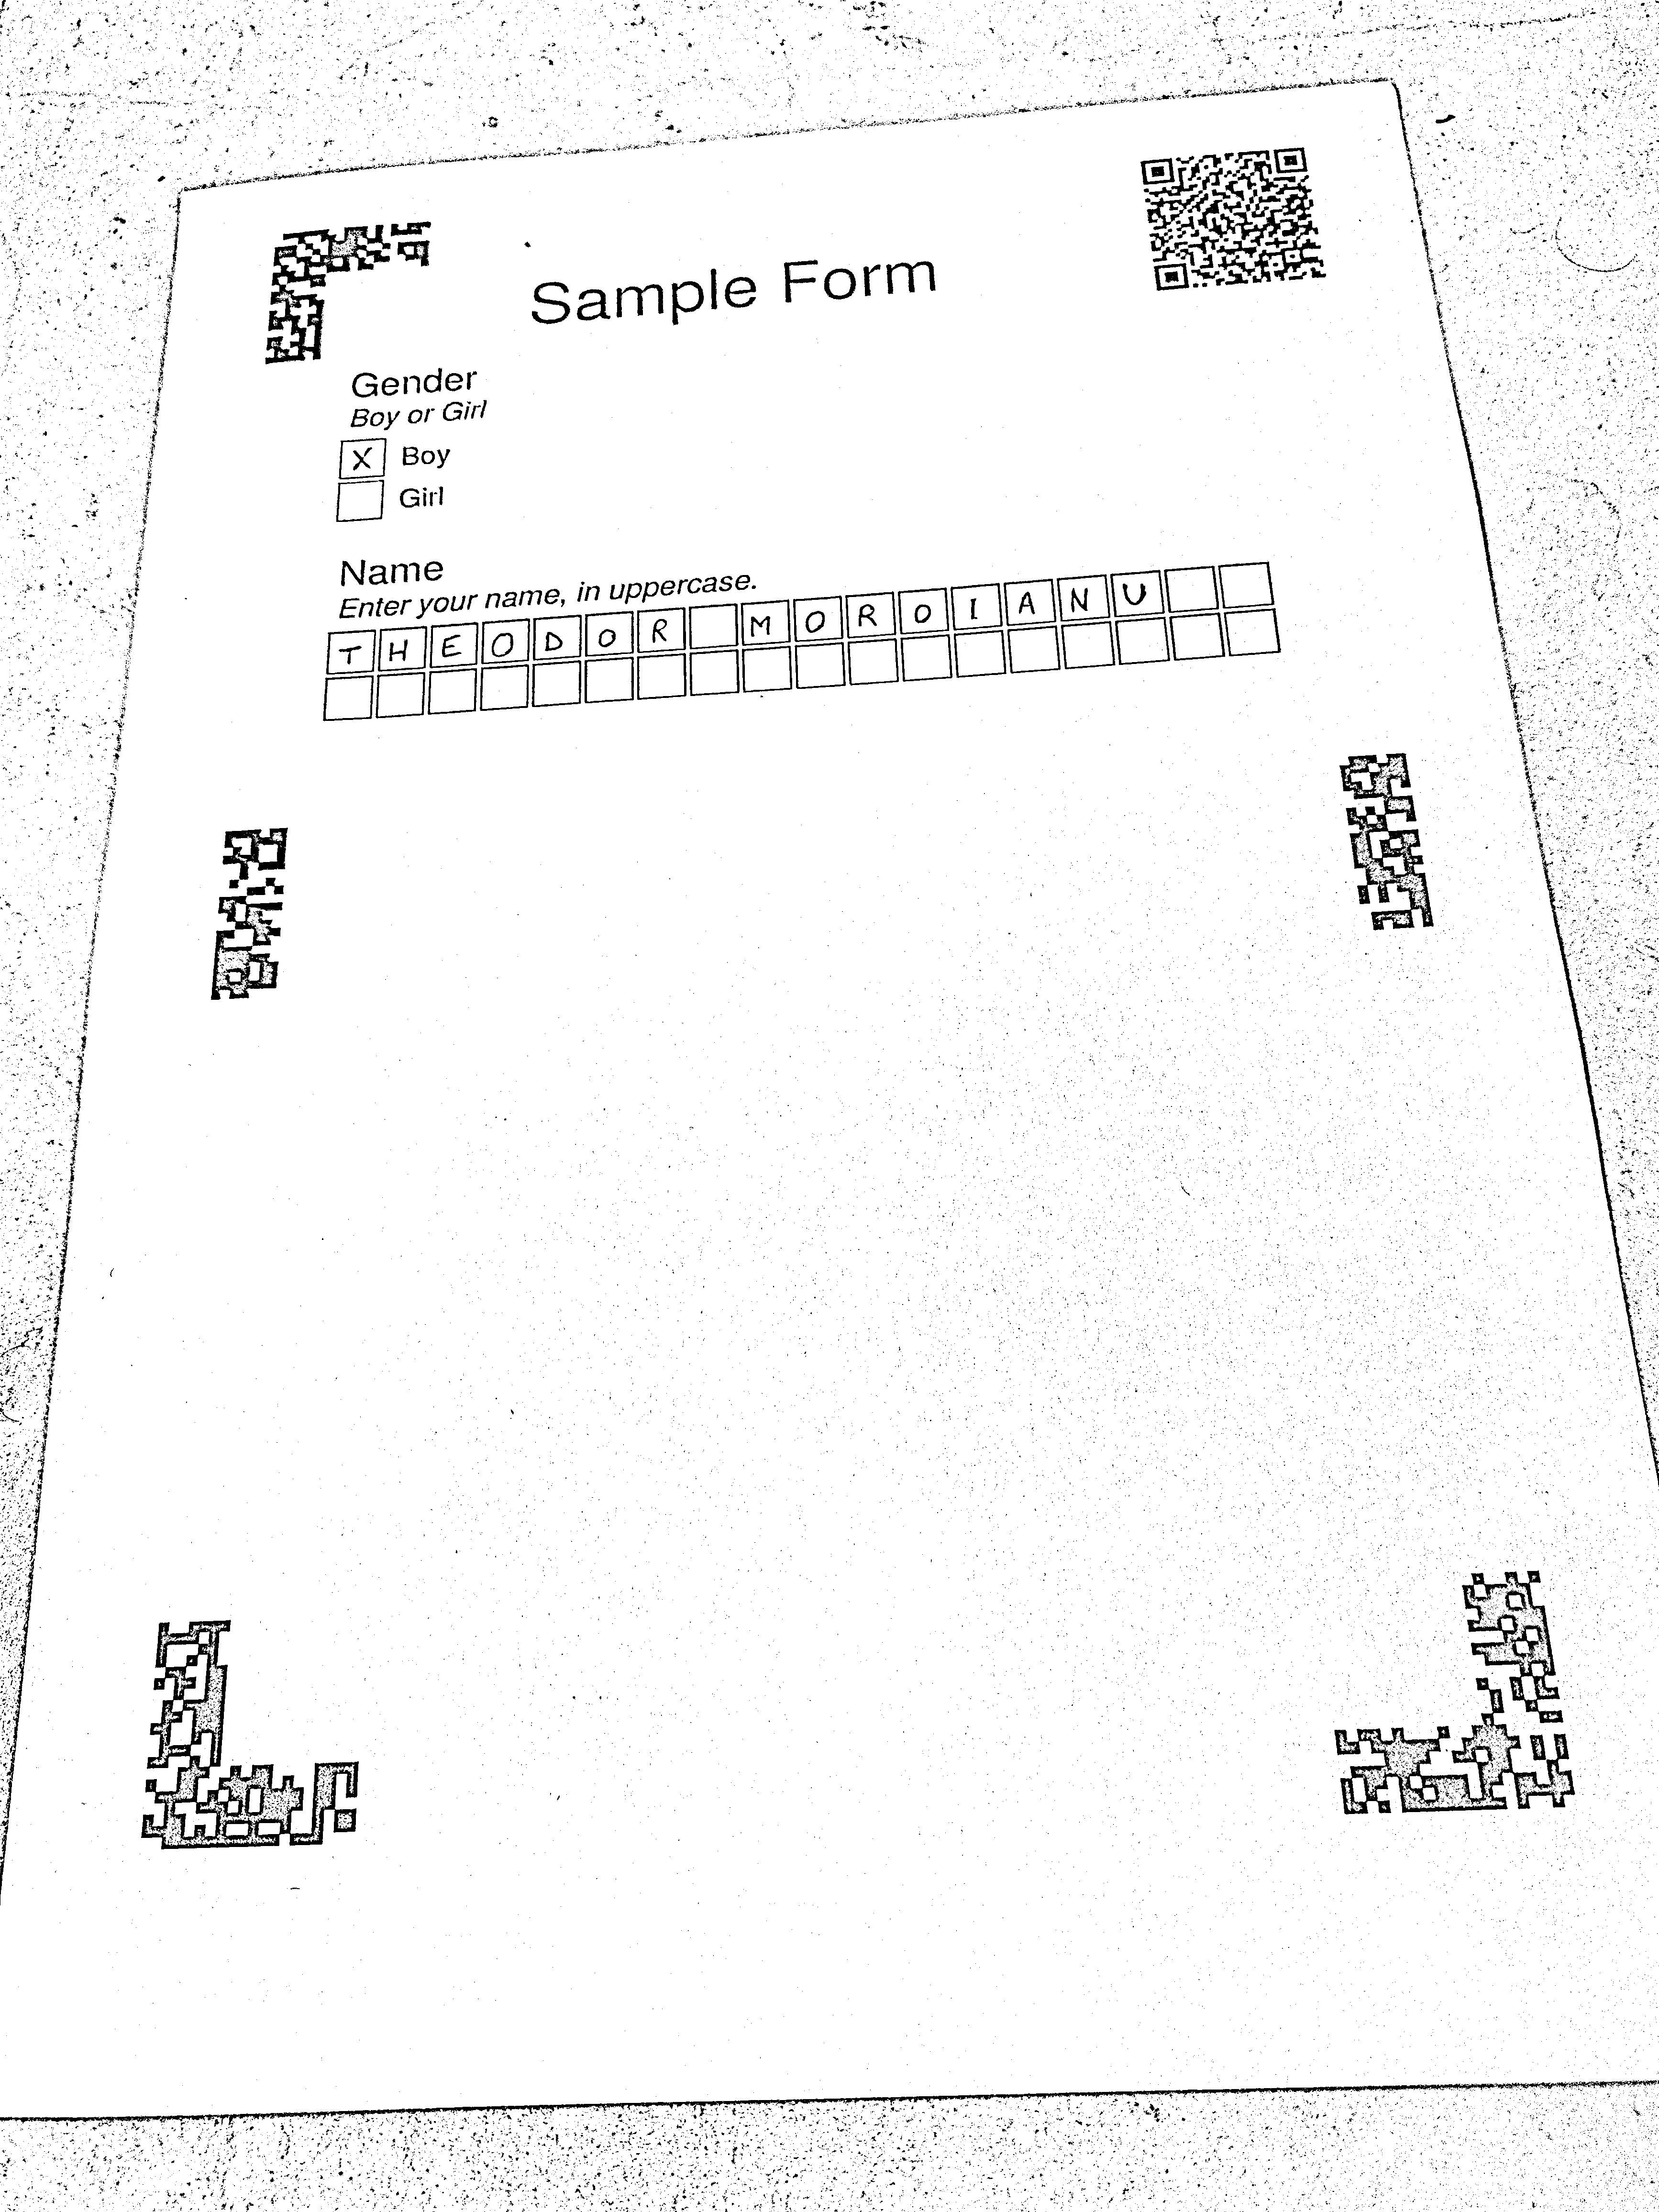
\includegraphics[width=5cm]{images/graphs/parser_processed_image.jpg} }}%
%     \caption{2 Figures side by side}%
%     %\label{fig:example}%
% \end{figure}

 \begin{figure}[!h]
     \centering
     \fbox{\includegraphics[width=35em]{images/graphs/parser_image_matches.png}}
     \caption{Matches found with ORB}
     \label{orb-matches}
 \end{figure}

For parsing the form, we have to be able to match specific pixels of the picture / scan of the form with the template, to figure out where locations we are interested in are. Further in this section, we will call the picture / scan of the form the \textit{picture}, and the original form, retrieved from the database, the \textit{template}.

Matching the picture with the template is not trivial, as things become quite messy:
\begin{itemize}
    \item If the picture keeps the same proportions, orientation and scaling as the template, then we have a perfect 1-1 match between the two.
    \item If the picture keeps the same proportions and orientation, but the scaling is not $1$, then a scaling factor is needed in order to be able to match the picture and the template.
    \item If the picture only keeps the same proportions, then in addition to the scaling factor a rotating factor is also required.
    \item If the picture does not keep the same proportions, then we have to find a homography between the two.
\end{itemize}

As finding homographies between two images is a quite common task, \textit{OpenCV} offers the ORB feature extractor\cite{rublee2011orb}, which is able to extract and match features of the two images, as seen in Figure \ref{orb-matches}. If enough matches are found, we can change the image's perspective, to get a frontal view of the form.


\begin{figure}[!h]
	\centering
	\fbox{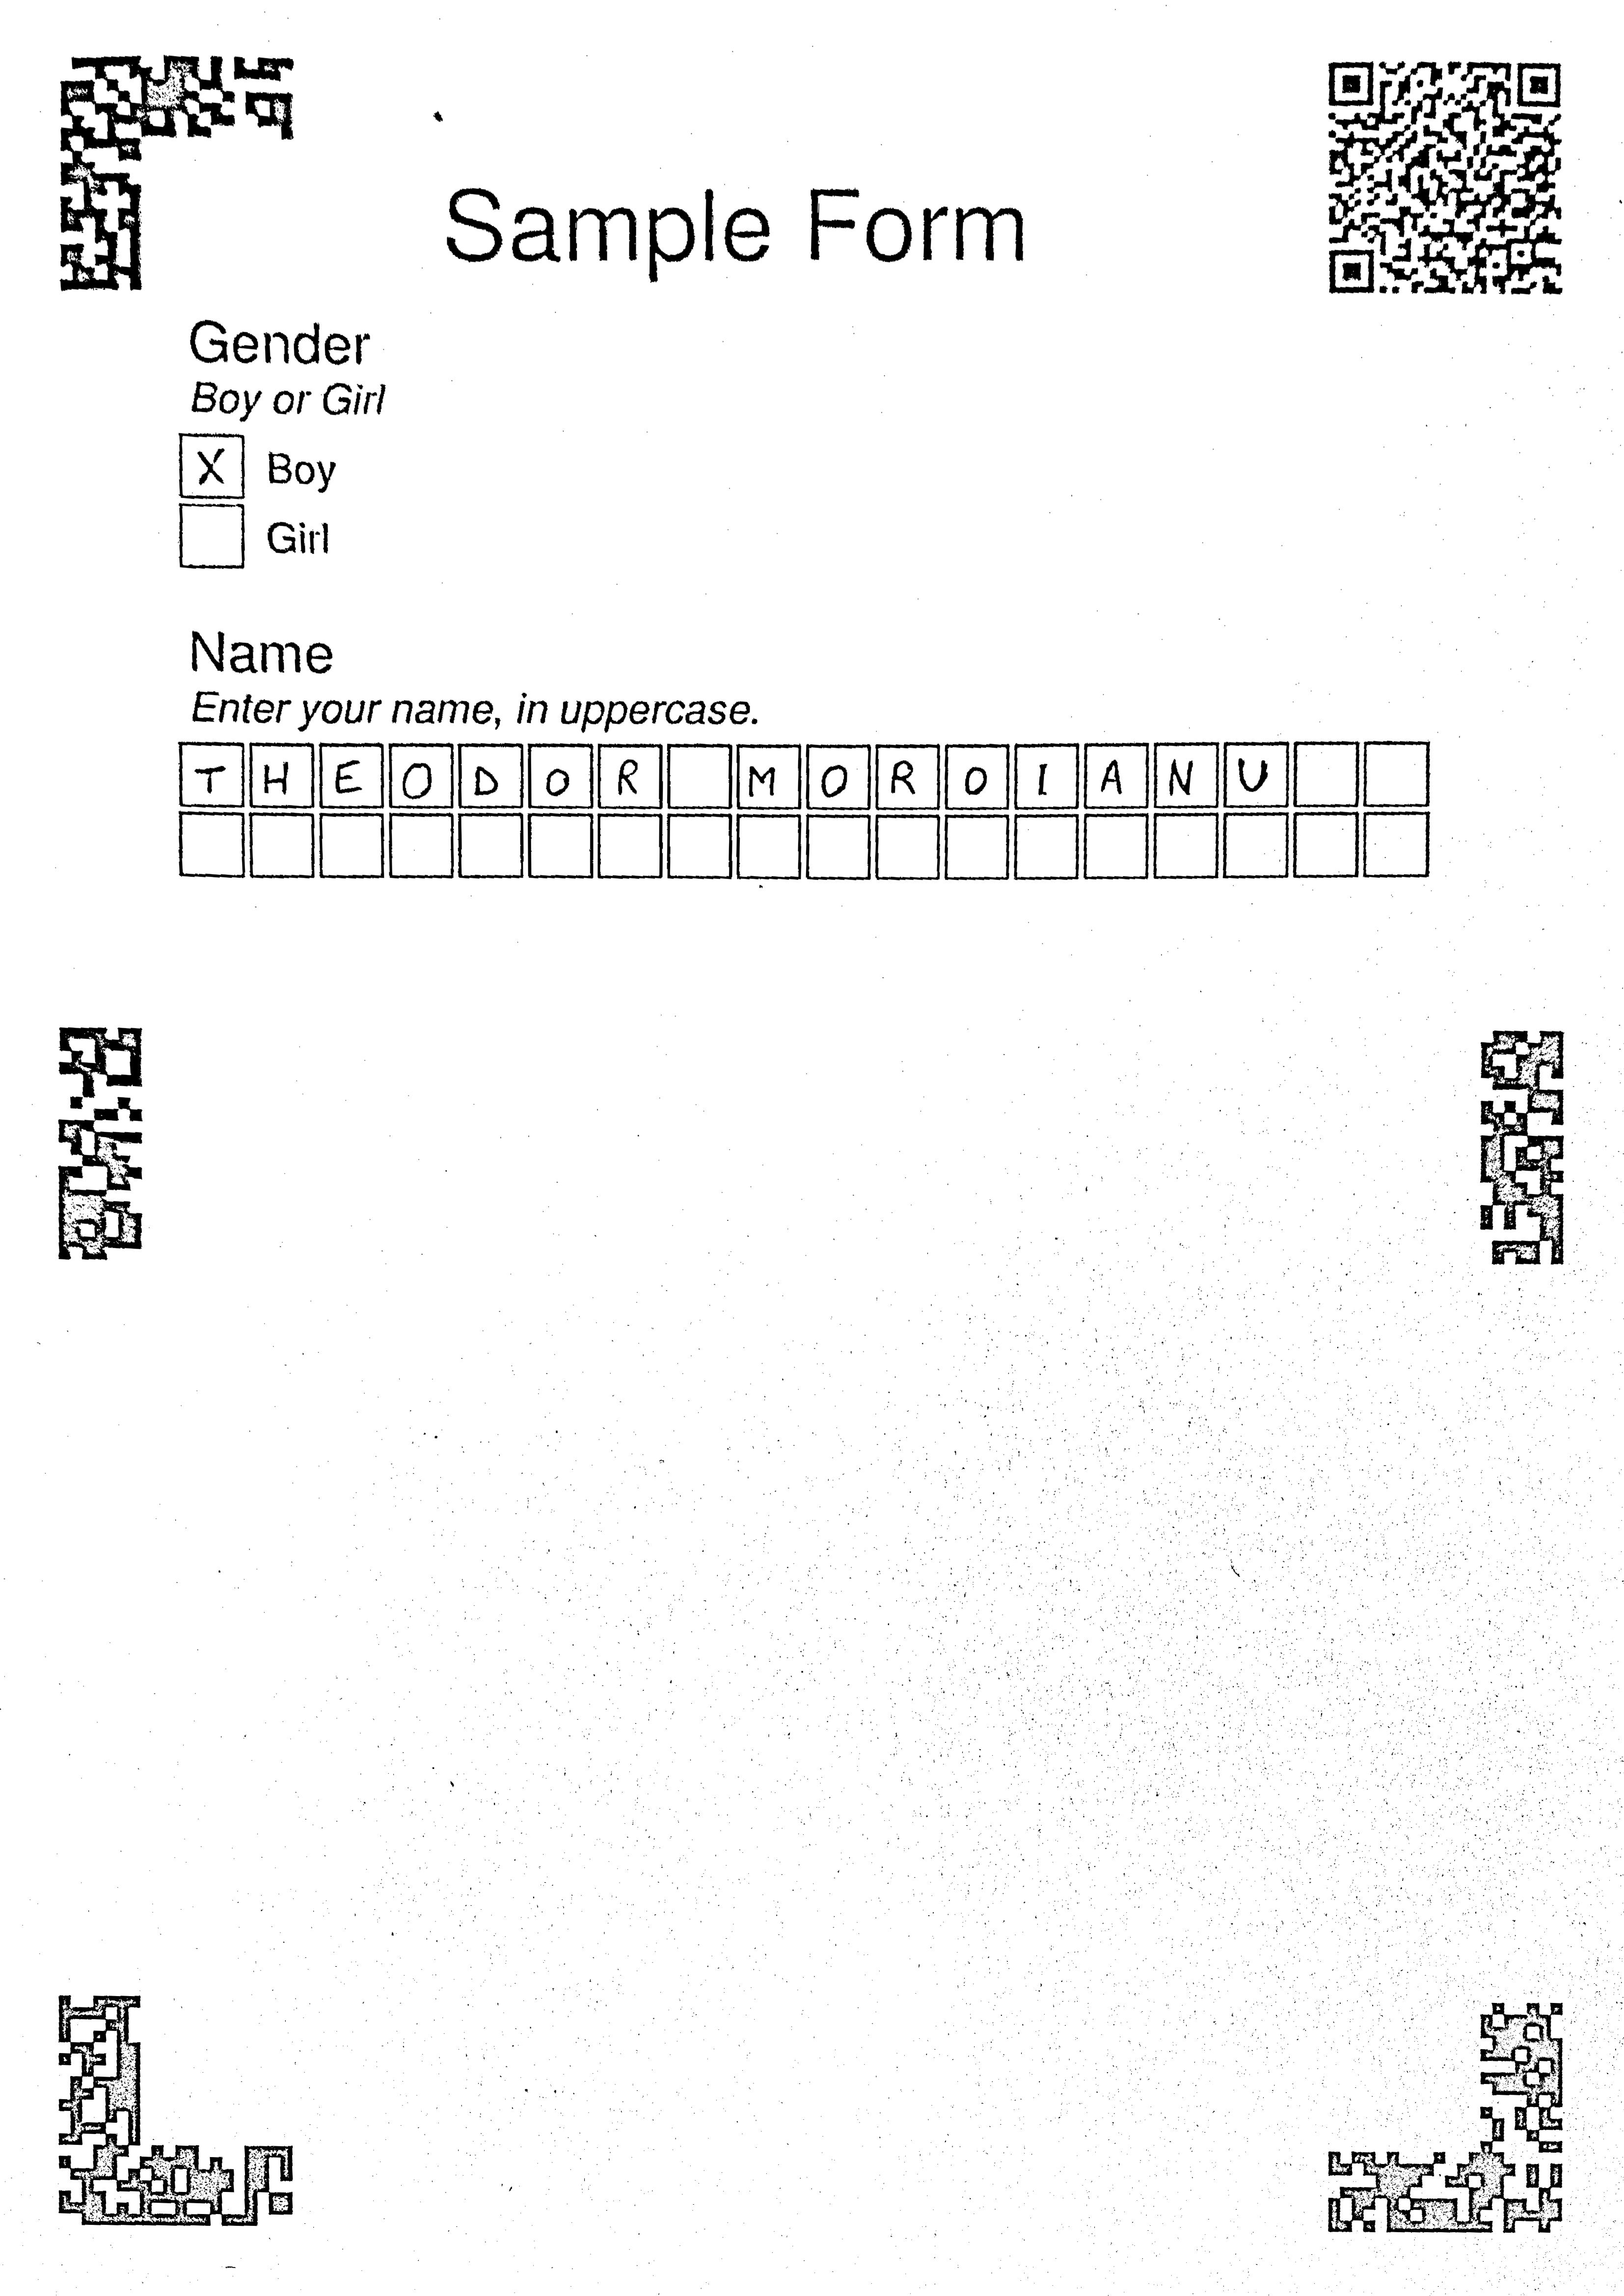
\includegraphics[width=15em]{images/graphs/parser_corrected_image.jpg}}
	\caption{Corrected Picture}
	\label{parser-corrected-image}
\end{figure}

In Figure \ref{parser-corrected-image} we can see the result of our perspective transformation over the binary picture. We can observe that:

\begin{itemize}
	\item The thresholding is not perfect, as some white areas have a few black pixels, and black text has a few white spots, which means that our OCR network has to be resistant to small noise.
	\item Straight lines (more specifically the boundaries of the text boxes) seem slightly curved. This is actually the case, as phone cameras add small distorsions to the images. This fenomenon does not appear on scans though.
\end{itemize}

\section{Extracting Answer Squares}

Extracting squares containing an answer from a form is straightforward, given a corrected image. As we save the position of squares where users are writing their answers when we generate the form, we simply have to extract said square.

For each form we store in the database a list with the absolute position of each answer square. An sample of the stored information is:

\begin{minted}[bgcolor=bg]{yaml}
    answer_squares_location:
        - 0:
            - 0:
                - width: 8
                - x: 23.5
                - y: 49.5
                - page: 0
            - 1:
                - width: 8
                - x: 32.5
                - y: 49.5
                - page: 0
            ...
        - 1:
            - 0:
                - width: 8
                - x: 23.5
                - y: 89.5
            ...
\end{minted}

With the help of the information mentioned above, and of a corrected image similar to Figure \ref{parser-corrected-image}, we can mark and extract each answer square of the form. We marked in Figure \ref{answer-squares-red} the answer squares we extract in red.

\begin{figure}[!h]
	\centering
	\fbox{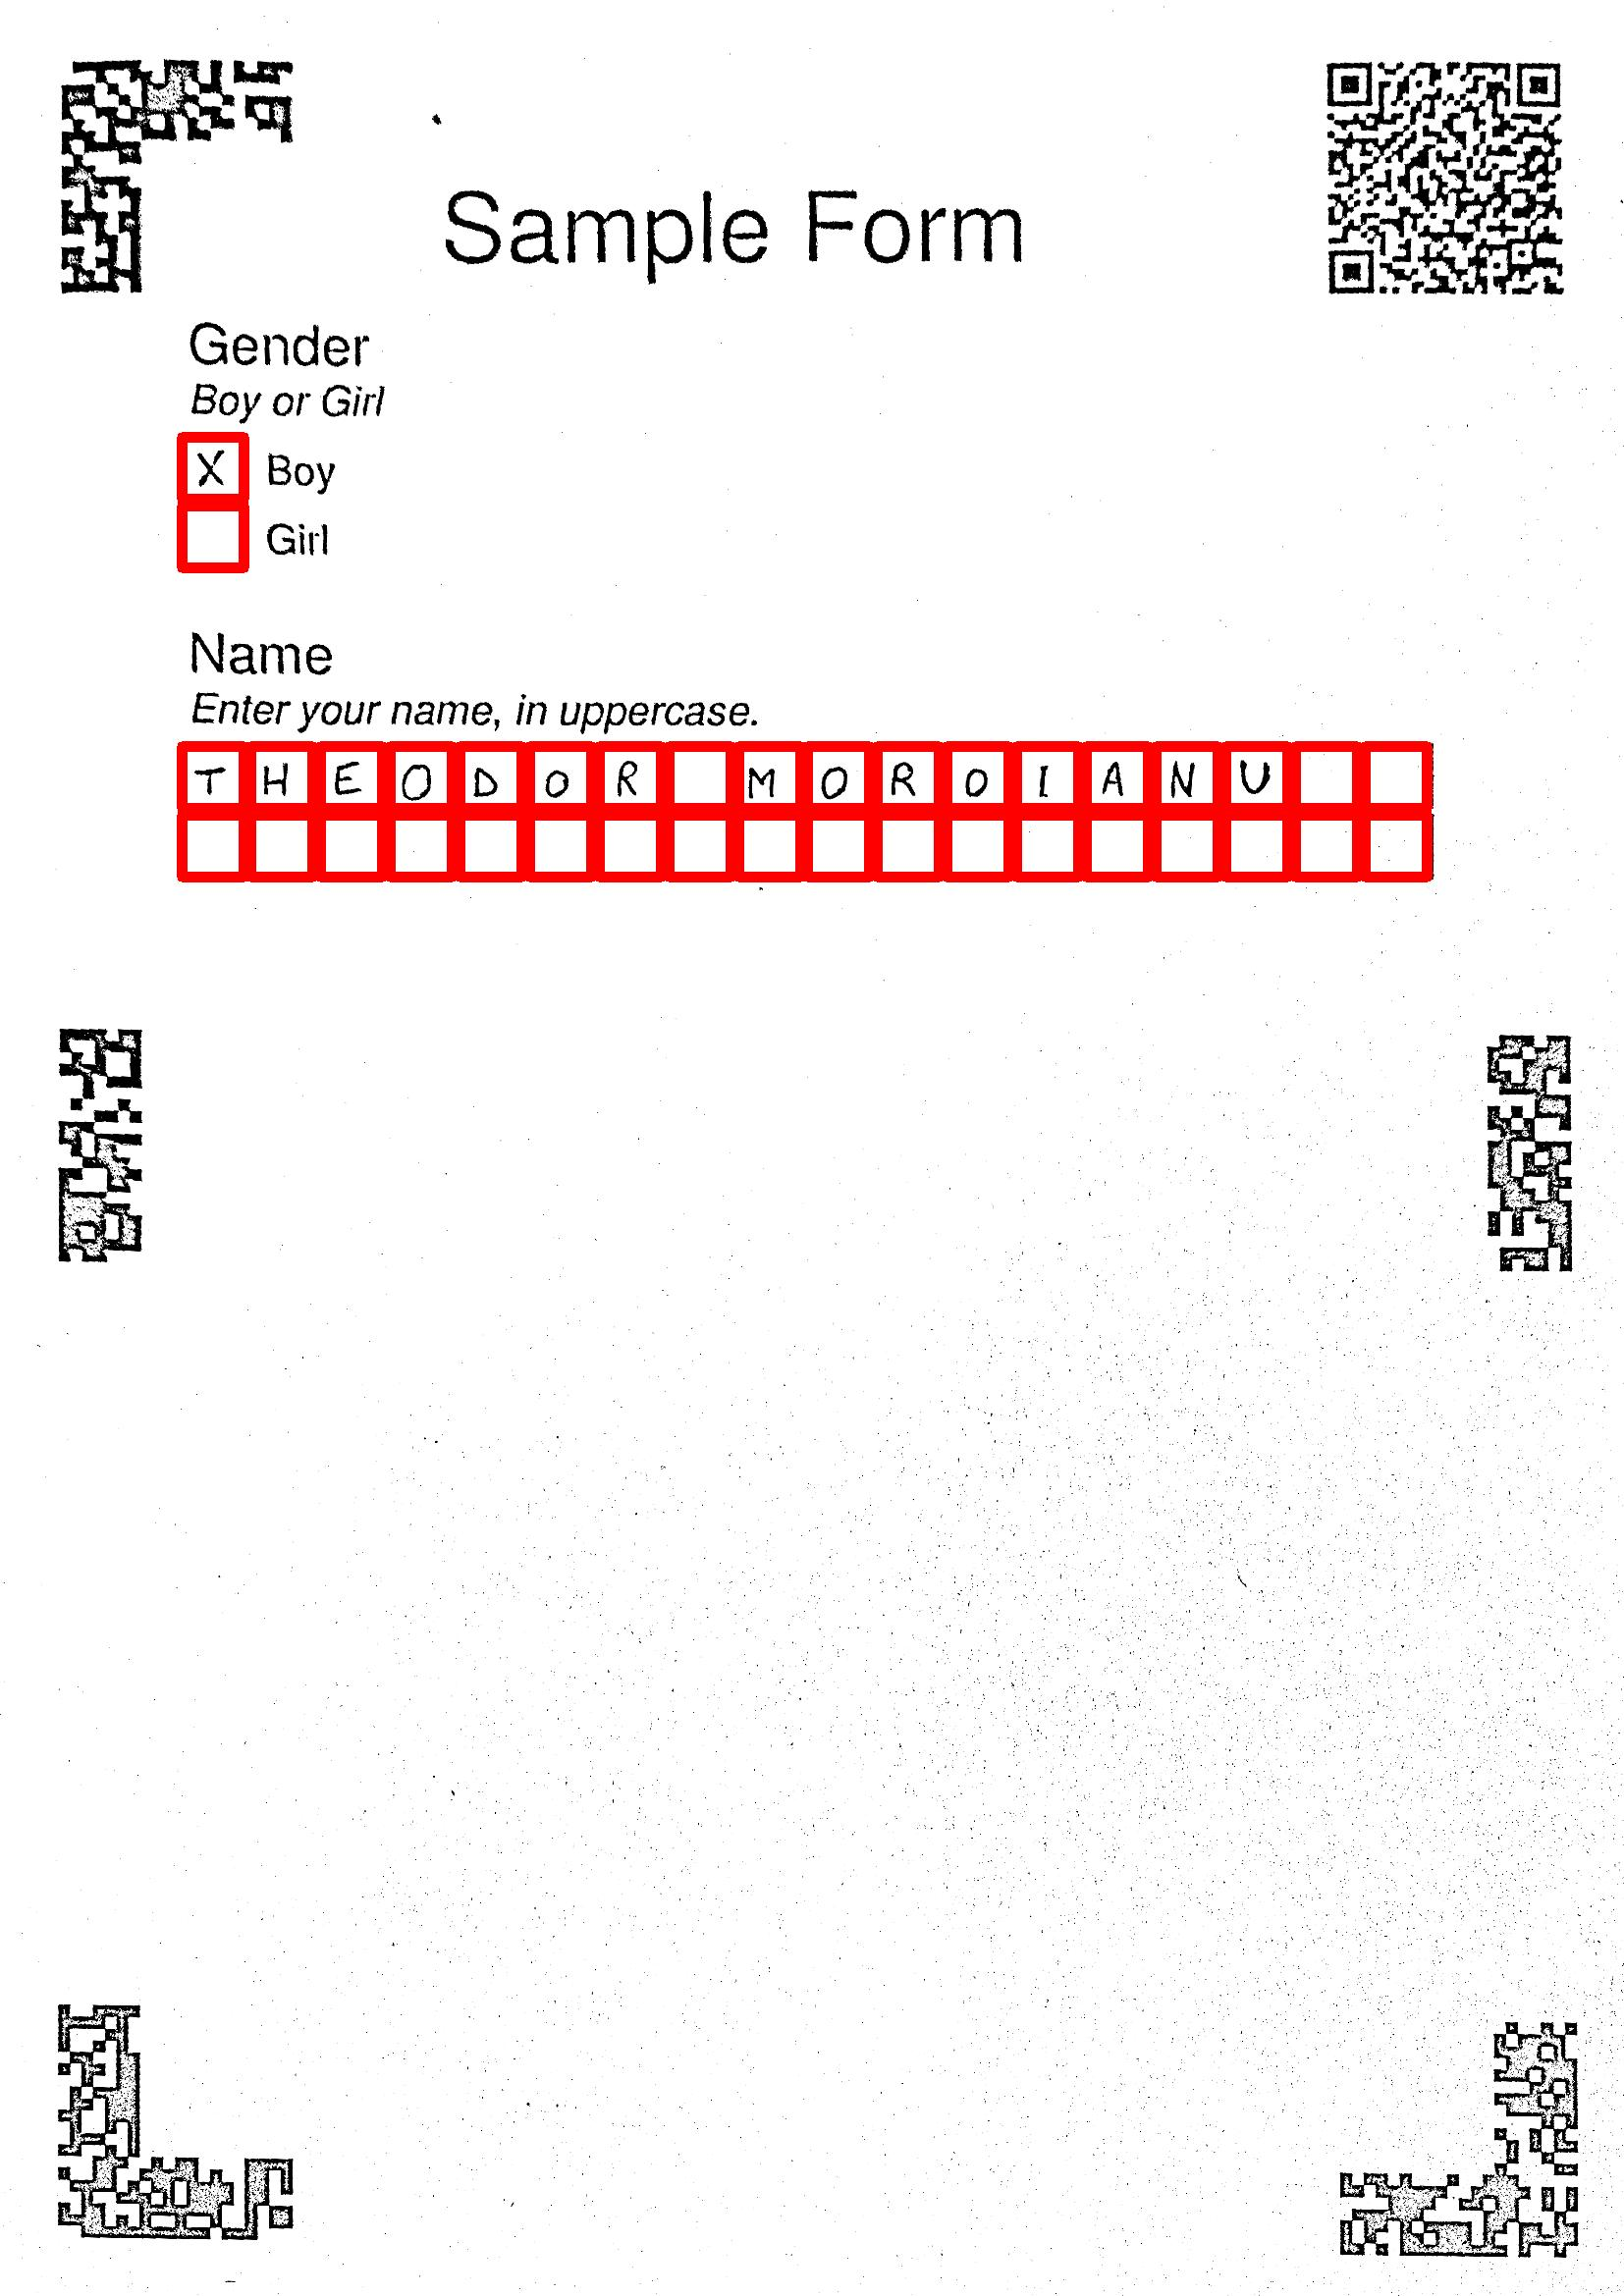
\includegraphics[width=18em]{images/graphs/fixed_image_squares.jpg}}
	\caption{Answer Squares Marked}
	\label{answer-squares-red}
\end{figure}

% cum antrenez reteaua
\chapter{Neural Network Design and Training}

\section{Why Use a CNN}

Using traditional CV approaches we have been able to isolate small images of the characters we want to extract. While traditional methods (such as HOG\cite{HOG} approaches) perform reasonably well, we decided to design, train and use a convolutional neural network (CNN)\cite{CNN}, which often outperforms classic classificators.

We use \textit{Pytorch}, "\textit{an optimized tensor library for deep learning using GPUs and CPU}"\cite{pytorch}. \textit{Pytorch} allows us to design, train, save and evaluate a convolutional neural network we then use to predict characters.

\section{CNN Architecture}

\section{Dataset Used}

\section{Data Processing and Augmentation}

\section{Training}

\section{Contiguous Training}


% Aici vorbesc despre fastapi, si cum il folosesc in aplicatie
\chapter{HTTP/S Server, Secure Authentication}

\section{FastAPI}

\section{Session Middleware}

\section{Oauth2}


% Vorbesc despre cum a functionat git, CI/CD, sincronizare cu Felix
\chapter{Tests, Source Control and CI/CD}

\section{Git}

\section{Smartforms Backend / Frontend}

\section{Testing}

\section{CI/CD}

% vorbesc de ce poate fi adaugat in plus
\chapter{Conclusion and Future Work}

Stuff that can be added to enhance the user experience:

Merge with conclusion

\begin{itemize}
    \item Add in the QR code info about the form, to not require a database.
    \item Add multi-threading while reading forms, to speed up the process. 23
\end{itemize}

\begin{thebibliography}{99}	

\bibitem{wicker1999reed}
S.~B.~Wicker, V.~K.~Bhargava,
\emph{Reed-Solomon codes and their applications},
John Wiley \& Sons, 1999.

\bibitem{masinter1998rfc2388}
L.~Masinter, 
\emph{RFC2388: Returning Values from Forms: multipart/form-data},
RFC Editor, 1998.

\bibitem{opencv-color-convention}
\emph{OpenCV: Color Conversions}, n.d., accessed 29 May 2022,  https://docs.opencv.org/3.4/de/d25/imgproc\_color\_conversions.html.

\bibitem{opencv-image-threshold}
\emph{OpenCV: Image Thresholding}, n.d., accessed 29 May 2022,
https://docs.opencv.org/4.x/d7/d4d/tutorial\_py\_thresholding.html

\bibitem{checker-illusion}
E.~H.~Adelson, Pbroks13, \emph{checker shadow illusion}, accessed 29 May 2022, https://commons.wikimedia.org/w/index.php?curid=75000950.

\bibitem{rublee2011orb}
E.~Rublee, V.~Rabaud, K.~Konolige, G.~Bradski,
\emph{ORB: An efficient alternative to SIFT or SURF},
	2011 International conference on computer vision, IEEE (2011),
	2564--2571.

\bibitem{HOG}
N.~Dalal, B.~Triggs,
\emph{Histograms of oriented gradients for human detection},
2005 IEEE computer society conference on computer vision and pattern recognition, IEEE (2005), Vol. 1, 886--893.

\bibitem{CNN}
K.~O'Shea, R.~Nash,
\emph{An introduction to convolutional neural networks},
arXiv:1511.08458, 2015.

\bibitem{pytorch}
\emph{Pytorch documentation}, n.d., accessed 30 May 2022,
https://pytorch.org/docs/stable/index.html.

\end{thebibliography}
%\printbibliography
%\printbibliography[heading=bibintoc]
\end{document}
